\documentclass[11pt,a4paper]{article}

\usepackage[T1]{fontenc}
\usepackage[utf8]{inputenc}
\usepackage[spanish,es-noshorthands]{babel}
\usepackage{lmodern}
\usepackage{amsmath,amssymb,amsthm}
\usepackage[margin=2.35cm]{geometry}
\usepackage{booktabs}
\usepackage{graphicx}
\usepackage{microtype}
\usepackage{enumitem}
\usepackage[colorlinks=true,linkcolor=black,citecolor=black,urlcolor=blue]{hyperref}

\graphicspath{{figuras_variantes/}}

\newcommand{\dd}{\,\mathrm{d}}
\newcommand{\p}{\partial}
\newcommand{\Rv}{\mathcal{R}_v}
\newcommand{\vin}{v_{\mathrm{in}}}
\newcommand{\pc}{\ifmmode\text{\,\%}\else\,\%\fi}
\newcommand{\MPa}{\ensuremath{\,\mathrm{MPa}}}
\newcommand{\ms}{\ensuremath{\,\mathrm{m/s}}}
\newcommand{\Pam}{\ensuremath{\,\mathrm{Pa/m}}}

\newtheorem{proposicion}{Proposición}

\title{\vspace{-1.2cm}\textbf{Conducto bifásico: ecuaciones y marchas}\\[0.25em]
\large Caso Calbuco 2015}
\author{Ignacio Gómez Gómez}
\date{\today}

\begin{document}
\maketitle
\vspace{-0.7cm}

\begin{abstract}\noindent
Se escriben las ecuaciones del conducto estacionario, primero en una
dimensión y después en el cilindro, y la reducción en la que las
velocidades radiales son nulas. En el tramo sin burbujas el momento
promediado sobre la parábola da la pendiente de presión con el divisor
de compresibilidad. Se fija el estado un metro sobre la saturación, se
parten los regímenes con el número capilar y se describe la marcha en
diferencias finitas. Al fragmentar se registran los cierres que ya se
integraron, con la cifra y la figura de cada corrida. Al final se
escribe el mismo conducto unidimensional con dependencia en el
tiempo, las condiciones que lo cierran y las escalas en las que
ese término pesa. El cilindro con dependencia angular es el
modelo tridimensional del que sale el eje-simétrico al anular
$\partial/\partial\theta$ y la velocidad angular.
\end{abstract}

\tableofcontents
\vspace{0.4em}

\section{Variables}

Tres cantidades distintas entran en la masa.

\paragraph{Variables.}
$\varphi$, fracción de volumen de gas, adimensional.
$N$, número de burbujas por unidad de volumen de fundido, en
$\mathrm{m^{-3}}$.
$n$, fracción másica de agua ya exsuelta.

$\varphi\in[0,1]$ es incógnita de campo: $\varphi(z)$ en el conducto
unidimensional y $\varphi(r,z)$ en el cilindro. Crece cuando las
burbujas crecen, aunque $N$ no cambie. La relación geométrica entre
ambas es
\begin{equation}
\label{eq:rb}
\varphi
=N\cdot\Bigl(\tfrac43\pi r_b^3\Bigr)\cdot(1-\varphi),
\qquad
r_b
=\Biggl(\frac{\varphi}{\tfrac43\pi N(1-\varphi)}\Biggr)^{1/3}.
\end{equation}
El mismo $\varphi$ con otro $N$ cambia $r_b$, y con él el arrastre y
la viscosidad.

$n=n(P,\xi)$ sale de Henry. Con $u_m=u_g$, el volumen compatible con
esa masa es
\begin{equation}
\label{eq:phi-noslip}
\varphi
=\Biggl(1+\frac{P}{n\,\Rv T}\frac{1-n}{\rho_m}\Biggr)^{-1}.
\end{equation}
Esa igualdad vale en la base, donde las dos fases van juntas. A lo
largo del conducto $u_g\neq u_m$ y $\varphi$ queda libre: lo cierran
la masa y el momento.

El resto del estado es la presión $P$, la cristalinidad $\xi$, las
velocidades verticales $u_m$ y $u_g$, y, en el cilindro, las radiales
$u_{m,r}$ y $u_{g,r}$. La densidad del fundido $\rho_m$ se toma
constante fuera del tramo sin burbujas. La del gas es la ecuación de
estado
\begin{equation}
\label{eq:eos}
\rho_g=\frac{P}{\Rv T}.
\end{equation}
Dado $P$, \eqref{eq:eos} da $\rho_g$. La presión la determina el
momento.

Caso de todas las marchas: cilindro de radio $R=16\,\mathrm{m}$,
base en $H=-7000\,\mathrm{m}$, $z$ hacia arriba,
$\varphi_{\mathrm{crit}}$ entre $0{,}525$ y $0{,}785$ según el
capilar, $P_{\mathrm{atm}}=10^{5}\,\mathrm{Pa}$,
$T=1173{,}15\,\mathrm{K}$, $\xi_0=0{,}25$,
$\tau_c=2\,\mathrm{h}$.

\section{Conducto unidimensional}
\label{sec:1d}

Dominio $z\in[H,0]$. El estado es
$(P,\varphi,N,\xi,u_m,u_g)(z)$. El caudal másico por unidad de área
$q$ es constante. El $\mathrm{MER}$ es $\pi R^2 q$. El valor de $q$
sale del tiro.

\subsection{Masa}

\paragraph{Variables.}
$\varphi$, $u_m$, $u_g$, y el escalar $q$. Entra $n=n(P,\xi)$.

Con sección constante el flujo másico no cambia con $z$:
\begin{equation}
\label{eq:q}
q
=\rho_m(1-\varphi)\,u_m
+\rho_g\,\varphi\,u_g
=\mathrm{const}.
\end{equation}
Se identifica $n$ con la fracción de ese flujo que va en el gas,
\begin{equation}
\label{eq:n-flux}
n
=\frac{\rho_g\,\varphi\,u_g}{q},
\qquad
1-n
=\frac{\rho_m(1-\varphi)\,u_m}{q}.
\end{equation}
De ahí se despejan las velocidades:
\begin{equation}
\label{eq:vel}
u_m
=\frac{q\,(1-n)}{(1-\varphi)\,\rho_m},
\qquad
u_g
=\frac{q\,n}{\varphi\,\rho_g}.
\end{equation}
$u_m$ y $u_g$ son algebraicas. En la base, $u_m=u_g=\vin$ y
$\varphi$ queda por \eqref{eq:phi-noslip}. Si $n=0$, entonces
$\varphi(H)=0$ y $q=\vin\rho_m$.

\subsection{\texorpdfstring{Momento, y la ecuación de $P$}{Momento, y la ecuación de P}}

\paragraph{Variables.}
$P$, $u_m$, $u_g$. Entran $\varphi$, el arrastre $F_{mg}$, el roce de
pared $F_{mw}$ y la viscosidad $\mu$ dentro de $F_{mw}$.

\begin{align}
\label{eq:mom-1d}
\rho_m(1-\varphi)\,u_m\frac{\dd u_m}{\dd z}
&=-(1-\varphi)\frac{\dd P}{\dd z}
-\rho_m(1-\varphi)\,g
+F_{mg}-F_{mw},
\\
\rho_g\varphi\,u_g\frac{\dd u_g}{\dd z}
&=-\varphi\frac{\dd P}{\dd z}
-\rho_g\varphi\,g
-F_{mg}-F_{gw}.
\end{align}
$F_{mw}=c_g\mu u_m/R^2$ antes de fragmentar y $F_{mw}=0$ después.
$F_{gw}=0$ antes de fragmentar. Al sustituir \eqref{eq:vel} el
sistema es lineal en $\dd P/\dd z$ y $\dd\varphi/\dd z$:
\begin{equation}
\label{eq:P-1d}
\frac{\dd P}{\dd z}
=\frac{-e\,a+f\,c}{ad-bc}
=:\mathcal{P}(P,\varphi,N,\xi;q),
\qquad
\frac{\dd\varphi}{\dd z}
=\frac{-e\,b+d\,f}{ad-bc}
=:\Phi(P,\varphi,N,\xi;q),
\end{equation}
\begin{align*}
a&=\rho_g u_g^2, &
b&=\varphi-\frac{u_g^2\varphi}{\Rv T}+\frac{\p n}{\p P}\,q\,u_g,\\
c&=\rho_m u_m^2, &
d&=\frac{\p n}{\p P}\,q\,u_m-(1-\varphi),\\
e&=-\rho_m(1-\varphi)\,g+F_{mg}-F_{mw}, &
f&=\rho_g\varphi\,g+F_{mg}+F_{gw}.
\end{align*}
La ecuación de la presión es \eqref{eq:P-1d}. En la base,
$P(H)=P_{\mathrm{lit}}+\Delta P=\rho_{\mathrm{crust}}g|H|+\Delta P$.
En la boca efusiva, $P(0)=P_{\mathrm{atm}}$ y
$\varphi(0)\le\varphi_{\mathrm{crit}}$. En la explosiva,
$P(0)=P_{\mathrm{atm}}$ o $u_g(0)\approx c_s=\sqrt{\Rv T}$, con
$\varphi(0)\ge\varphi_{\mathrm{crit}}$.

\subsection{\texorpdfstring{Transporte de $N$ y de $\xi$}{Transporte de N y de xi}}

\paragraph{Variables de $N$.}
$N$. Entran $\varphi$ y $\mu$ a través de $r_b$ y de la coalescencia.

\begin{equation}
\label{eq:N-1d}
\frac{\dd N}{\dd z}
=\frac{1}{u_m}\Gamma_N(P,\varphi,N,\xi).
\end{equation}
$\Gamma_N\le 0$ es la coalescencia de Slezin. Se anula si
$r_b\ge R/2$ o $\varphi\ge\varphi_{\mathrm{crit}}$. Después de
fragmentar, $N$ queda en el valor del cruce. En la base,
$N(H)=10^{8}\,\mathrm{m^{-3}}$ si no hay exsolución; si la hay,
Toramaru da $\log_{10}N=1{,}5\log_{10}\dot P+5$ con
$\dot P=-(\dd P/\dd z)\,\vin$.

\paragraph{Variables de $\xi$.}
$\xi$. Entra $P$ por el equilibrio.

\begin{equation}
\label{eq:xi-1d}
\frac{\dd\xi}{\dd z}
=\frac{1}{u_m}\Gamma_\xi(P,\xi),
\qquad
\Gamma_\xi
=\max\Bigl(0,\;
(\xi_{\max}-\xi_0)\,f_2 f_3/\tau_c\Bigr).
\end{equation}
$f_2$ y $f_3$ interpolan hacia $\xi_{\mathrm{eq}}(P)$. Después de
fragmentar, $\xi$ queda en el valor del cruce. En la base,
$\xi(H)=\xi_0$.

\subsection{Henry, arrastre y viscosidad}

\paragraph{Variables.}
$n(P,\xi)$, $F_{mg}(\varphi,u_g-u_m,r_b,\mu,\rho_g)$ y
$\mu(P,\varphi,\xi,N,u_m)$.

\begin{equation}
\label{eq:henry}
n(P,\xi)
=\max\Biggl(0,\;
\frac{(1-\xi_0)c_0-(1-\xi)\,C_1 P^{\beta}}{1-C_1 P^{\beta}}\Biggr).
\end{equation}
$r_b$ es \eqref{eq:rb}. El Reynolds de la burbuja es
$Re_b=2r_b\rho_g|u_g-u_m|/\mu_g$ con
$\mu_g=10^{-5}\,\mathrm{Pa\,s}$.

Los umbrales $\varphi_1<\varphi_2<\varphi_{\mathrm{crit}}$ se
calculan una vez por tiro, en el estado $\varphi^\ast=0{,}2$. Se
busca $P^\ast\in[P_{\mathrm{atm}},P_{\mathrm{sat}}]$ tal que la
fracción de Henry quede a menos de $0{,}002$ de $0{,}2$. Ahí
\begin{equation}
\label{eq:Ca-ast}
\begin{aligned}
\dot\gamma_\ast
&=\frac12\Biggl(
\vin
\frac{
-\partial_P n\,\partial_z P\,(1-\varphi^\ast)
+(1-n)\,\partial_P\varphi\,\partial_z P
}{(1-\varphi^\ast)^2}
+\frac{\vin}{R}
\Biggr),
\\
Ca_\ast
&=\bigl\lvert\dot\gamma_\ast\,\mu_\ast\,r_{b,\ast}/0{,}3\bigr\rvert.
\end{aligned}
\end{equation}
Con $\varphi_{\mathrm{sup}}=0{,}785$,
$\varphi_{\mathrm{inf}}=0{,}525$,
$\varphi_{\mathrm{per}}^-=0{,}15$ y
$\varphi_{\mathrm{per}}^+=0{,}40$,
\begin{equation}
\label{eq:umbrales-Ca}
\begin{aligned}
\varphi_{\mathrm{crit}}
&=\frac{\varphi_{\mathrm{sup}}-\varphi_{\mathrm{inf}}}{2}\,
\mathrm{erf}(\log_{10}Ca_\ast)
+\frac{\varphi_{\mathrm{sup}}+\varphi_{\mathrm{inf}}}{2},
\\
\varphi_1
&=\frac{\varphi_{\mathrm{per}}^--\varphi_{\mathrm{per}}^+}{2}\,
\mathrm{erf}(\log_{10}Ca_\ast)
+\frac{\varphi_{\mathrm{per}}^-+\varphi_{\mathrm{per}}^+}{2},
\\
\varphi_2
&=\varphi_1+0{,}01.
\end{aligned}
\end{equation}
Así $\varphi_{\mathrm{crit}}\in[0{,}525,\,0{,}785]$ y
$\varphi_1\in[0{,}15,\,0{,}40]$. $Ca_\ast\to 0$ da el piso y
$Ca_\ast\to\infty$ da el techo. Esos tres números parten
$[H,0]$ en
\begin{equation}
\label{eq:tramos}
\begin{aligned}
J_1&=\{z:\;0\le\varphi<\varphi_1\},&
J_2&=\{z:\;\varphi_1\le\varphi<\varphi_2\},\\
J_3&=\{z:\;\varphi_2\le\varphi<\varphi_{\mathrm{crit}}\},&
J_4&=\{z:\;\varphi\ge\varphi_{\mathrm{crit}}\}.
\end{aligned}
\end{equation}
El estado es continuo al cruzar $\varphi_k$. Cambia la fórmula de
$F_{mg}$. En $J_4$ se apaga $F_{mw}$, aparece $F_{gw}$ y se congelan
$N$ y $\xi$.

En $J_1$, Stokes:
\begin{equation}
\label{eq:Fmg1}
F_{mg}
=\frac{3\mu}{r_b^2}\,(u_g-u_m)\,\varphi(1-\varphi).
\end{equation}
En $J_2$, $\theta=(\varphi-\varphi_1)/(\varphi_2-\varphi_1)$. Si
$Re_b\le 2200$, con
$k=0{,}131\,r_b^2(\varphi-\varphi_1+0{,}05)^{2{,}1}$,
\begin{equation}
\label{eq:Fmg2}
F_{mg}
=\Biggl(\frac{\mu_g}{k}\Biggr)^\theta
\Biggl(\frac{3\mu}{r_b^2}\Biggr)^{1-\theta}
(u_g-u_m)\,\varphi(1-\varphi).
\end{equation}
Si $Re_b>2200$, el factor $\mu_g/k$ se reemplaza por
$0{,}33\rho_g|u_g-u_m|/(4r_b)$. En $J_3$ queda el extremo
$\theta=1$. En $J_4$, con $r_a=10^{-3}\,\mathrm{m}$ y $c_d=0{,}8$,
si $\varphi\ge\varphi_{\mathrm{crit}}+0{,}05$,
\begin{equation}
\label{eq:Fmg4}
F_{mg}
=\frac{3c_d}{8r_a}\,\rho_g\,|u_g-u_m|(u_g-u_m)\,\varphi(1-\varphi),
\end{equation}
y en la capa de ancho $0{,}05$ se interpola con $J_3$. Ahí
$F_{gw}=0{,}01\,\rho_g|u_g|u_g/(4R)$.

La viscosidad tiene tres factores. El fundido es Giordano,
$\mu_\ell=\mu_{\mathrm{Gio}}(c_d,T,X)$, con $T$ y la composición
anhidra fijas. El agua disuelta es $c_d=C_1 P^\beta$ si hay gas y
$c_d=c_0$ si no, así que $\mu_\ell=\mu_\ell(P)$. Los cristales, con
$\dot\gamma=u_m/R$, dan
\begin{equation}
\label{eq:thxi}
\theta_\xi
=\Bigl(1-\frac{\xi_0}{\phi_{\max,1}}\Bigr)^{-2{,}5}
\Bigl(1-\frac{\xi-\xi_0}{(1-\xi_0)\phi_{\max,2}}\Bigr)^{-2{,}5},
\end{equation}
$\phi_{\max,i}=0{,}656\exp\bigl(-(\log_{10}r_i)^2/(2\cdot 1{,}08^2)\bigr)$,
$r_1=4$, $r_2=8$. Las burbujas entran por Llewellin. Con
$Ca=r_b\mu_\ell\dot\gamma/3$,
$\varphi_\ast=\varphi_{\mathrm{crit}}+0{,}05$,
$A=(1-\varphi/\varphi_\ast)^{-\varphi_\ast}$,
$B=(1-\varphi/\varphi_\ast)^{5\varphi_\ast/3}$,
$c_1=-0{,}2895\,\varphi+0{,}8132$ y $c_2=\varphi$,
\begin{equation}
\label{eq:mu}
\mu
=\Biggl(\tfrac12(A-B)\bigl(1-\mathrm{erf}(c_1\log Ca+c_2)\bigr)+B\Biggr)
\theta_\xi\,\mu_\ell.
\end{equation}

El sistema, ya compuesto, es
\begin{equation}
\label{eq:dae}
\begin{aligned}
\frac{\dd P}{\dd z}
&=\mathcal{P}(P,\varphi,N,\xi;q),
&
\frac{\dd\varphi}{\dd z}
&=\Phi(P,\varphi,N,\xi;q),
\\
\frac{\dd N}{\dd z}
&=\frac{1}{u_m}\Gamma_N(P,\varphi,N,\xi,\mu),
&
\frac{\dd\xi}{\dd z}
&=\frac{1}{u_m}\Gamma_\xi(P,\xi).
\end{aligned}
\end{equation}
$P$ entra en $n$, en $\rho_g$ y en $\mu_\ell$. $\varphi$ entra en las
velocidades, en $F_{mg}$, en $\mu$ y en el tramo $J_k$. $N$ entra en
$r_b$. $\xi$ entra en Henry y en $\theta_\xi$. $u_m$ entra en
$\dot\gamma$ y divide las dos tasas. $q$ entra en \eqref{eq:vel} y lo
fija la boca.

En el código unidimensional, \eqref{eq:dae} es el DAE
$M\mathbf{y}'=F(\mathbf{y})$ con
$M=\mathrm{diag}(1,1,1,1,0,0)$, porque $u_m$ y $u_g$ son
algebraicas. Lo integra IDA con paso interno variable. La malla de
salida es independiente de esos pasos. Al cruzar
$\varphi_1$, $\varphi_2$ o $\varphi_{\mathrm{crit}}$ se corta el
tramo y se reinicia el integrador.

\section{Conducto bidimensional}
\label{sec:2d}

Cilindro $0\le r\le R$, $H\le z\le 0$. Las incógnitas dependen de
$(r,z)$.

\subsection{Masa}

\paragraph{Variables.}
$\varphi$, $u_m$, $u_g$, $u_{m,r}$, $u_{g,r}$. Entra la tasa de
exsolución $\Gamma$.

\begin{align}
\label{eq:masa-2d}
\frac{1}{r}\frac{\p}{\p r}\bigl(r\,\rho_m(1-\varphi)\,u_{m,r}\bigr)
+\frac{\p}{\p z}\bigl(\rho_m(1-\varphi)\,u_m\bigr)
&=-\Gamma,
\\
\frac{1}{r}\frac{\p}{\p r}\bigl(r\,\rho_g\varphi\,u_{g,r}\bigr)
+\frac{\p}{\p z}\bigl(\rho_g\varphi\,u_g\bigr)
&=\Gamma.
\end{align}
El caudal total es constante en $z$:
\begin{equation}
\label{eq:Q}
Q
=\int_0^R 2\pi r\bigl[
\rho_m(1-\varphi)\,u_m+\rho_g\,\varphi\,u_g
\bigr]\,\dd r.
\end{equation}
Dentro del conducto $\varphi$ sale de \eqref{eq:masa-2d} junto con
el momento. La fórmula \eqref{eq:phi-noslip} se usa en la base, donde
$u_m=u_g$. Si se identifica $n$ con la fracción local del flujo,
\begin{equation}
\label{eq:n-loc}
n
=\frac{\rho_g\,\varphi\,u_g}
{\rho_m(1-\varphi)\,u_m+\rho_g\,\varphi\,u_g},
\end{equation}
eso despeja velocidades, del mismo modo que \eqref{eq:vel}. En el
eje y en la pared, $u_{m,r}=u_{g,r}=0$.

\subsection{\texorpdfstring{Momento y la ecuación de $P$}{Momento y la ecuación de P}}

\paragraph{Variables.}
$P(r,z)$, $u_m$, $u_g$, $u_{m,r}$, $u_{g,r}$. Entran $\varphi$,
$\mu$, $\mu_g$ y $F_{mg}$.

En la dirección vertical,
\begin{align}
\label{eq:mom-mz}
\rho_m(1-\varphi)\Biggl(
u_{m,r}\frac{\p u_m}{\p r}+u_m\frac{\p u_m}{\p z}
\Biggr)
&=
-(1-\varphi)\frac{\p P}{\p z}
-\rho_m(1-\varphi)\,g
+F_{mg}
\nonumber\\
&\quad
+\frac{1}{r}\frac{\p}{\p r}\Biggl[
r\,\mu(1-\varphi)\frac{\p u_m}{\p r}
\Biggr]
+\frac{\p}{\p z}\Biggl[
\mu(1-\varphi)\frac{\p u_m}{\p z}
\Biggr],
\\
\label{eq:mom-gz}
\rho_g\varphi\Biggl(
u_{g,r}\frac{\p u_g}{\p r}+u_g\frac{\p u_g}{\p z}
\Biggr)
&=
-\varphi\frac{\p P}{\p z}
-\rho_g\varphi\,g
-F_{mg}
\nonumber\\
&\quad
+\frac{1}{r}\frac{\p}{\p r}\Biggl[
r\,\mu_g\varphi\frac{\p u_g}{\p r}
\Biggr]
+\frac{\p}{\p z}\Biggl[
\mu_g\varphi\frac{\p u_g}{\p z}
\Biggr].
\end{align}
Pasado el viscoseo al otro lado, la presión cumple
\begin{equation}
\label{eq:P-2d}
\begin{aligned}
(1-\varphi)\frac{\p P}{\p z}
&=
-\rho_m(1-\varphi)\Biggl(
u_{m,r}\frac{\p u_m}{\p r}+u_m\frac{\p u_m}{\p z}
\Biggr)
-\rho_m(1-\varphi)\,g
+F_{mg}
\\
&\quad
+\frac{1}{r}\frac{\p}{\p r}\Biggl[
r\,\mu(1-\varphi)\frac{\p u_m}{\p r}
\Biggr]
+\frac{\p}{\p z}\Biggl[
\mu(1-\varphi)\frac{\p u_m}{\p z}
\Biggr],
\\[0.35em]
(1-\varphi)\frac{\p P}{\p r}
&=
-\rho_m(1-\varphi)\Biggl(
u_{m,r}\frac{\p u_{m,r}}{\p r}+u_m\frac{\p u_{m,r}}{\p z}
\Biggr)
\\
&\quad
+\frac{1}{r}\frac{\p}{\p r}\Biggl[
r\,\mu(1-\varphi)\frac{\p u_{m,r}}{\p r}
\Biggr]
-\mu(1-\varphi)\frac{u_{m,r}}{r^2}
+\frac{\p}{\p z}\Biggl[
\mu(1-\varphi)\frac{\p u_{m,r}}{\p z}
\Biggr].
\end{aligned}
\end{equation}
La ecuación de $P$ es \eqref{eq:P-2d}. Al integrar el viscoseo hasta
la pared,
\begin{equation}
\label{eq:Fmw}
F_{mw}
=-\frac{2}{R}\Biggl[\mu(1-\varphi)\frac{\p u_m}{\p r}\Biggr]_{r=R},
\quad
F_{gw}
=-\frac{2}{R}\Biggl[\mu_g\varphi\frac{\p u_g}{\p r}\Biggr]_{r=R}.
\end{equation}
En la ecuación diferencial esos términos están en la condición
$u_m(R,z)=0$. En el eje, $\p u_m/\p r=\p u_g/\p r=\p P/\p r=0$.
En la base, $P(r,H)=P_{\mathrm{lit}}+\Delta P$. En la boca,
$P(r,0)=P_{\mathrm{atm}}$, o $u_g\approx c_s$ en el caso explosivo.

\subsection{Transporte y tasas}

\paragraph{Variables.}
$N(r,z)$ y $\xi(r,z)$. Entran $u_m$, $u_{m,r}$, $\Gamma_N$ y
$\Gamma_\xi$.

\begin{align}
\label{eq:Nxi-2d}
u_{m,r}\frac{\p N}{\p r}+u_m\frac{\p N}{\p z}
&=\Gamma_N,
\\
u_{m,r}\frac{\p \xi}{\p r}+u_m\frac{\p \xi}{\p z}
&=\Gamma_\xi.
\end{align}
En el eje, $\p N/\p r=\p\xi/\p r=0$. En la base, $N=N_0$ y
$\xi=\xi_0$.

La exsolución acopla la masa con $P$ y $\xi$. El flujo másico local
es $\mathbf{j}=\rho_m(1-\varphi)\mathbf{u}_m+\rho_g\varphi\mathbf{u}_g$.
Con $\nabla\cdot\mathbf{j}=0$ y $n=n(P,\xi)$,
\begin{equation}
\label{eq:Gamma}
\Gamma
=\mathbf{j}\cdot\nabla n
=j_r\frac{\p n}{\p r}+j_z\frac{\p n}{\p z},
\qquad
\nabla n
=\frac{\p n}{\p P}\nabla P+\frac{\p n}{\p\xi}\nabla\xi.
\end{equation}
$\Gamma$ entra en \eqref{eq:masa-2d}. Si $n$ es constante a lo largo
de $\mathbf{j}$, $\Gamma=0$.

La coalescencia, mientras $r_b<R/2$ y $\varphi<\varphi_{\mathrm{crit}}$,
es
\begin{equation}
\label{eq:GammaN}
\begin{aligned}
\Gamma_N
&=-N^{2/3}(1-\varphi)^{-1/3}
\cdot\frac19\frac{(\rho_m-\rho_g)g}{\mu}
\cdot\Biggl(\frac{3\varphi}{4\pi}\Biggr)^{2/3}
\\
&\quad\cdot(F_1^2-F_2^2)
\Biggl(1-(F_1+F_2)
\Biggl(\frac{3\varphi\cdot\pi/(6\varphi_{\mathrm{crit}})}{4\pi}\Biggr)^{1/3}
\Biggr)^{-1}
\\
&\quad\cdot F_c\,(1-\varphi/\varphi_{\mathrm{crit}})\,(R-r_b)/R,
\end{aligned}
\end{equation}
con $F_1=1{,}8$, $F_2=0{,}2$ y $F_c\in[0,1]$. Fuera de ese rango, y
después de fragmentar, $\Gamma_N=0$. Entra $\mu$, así que
$\Gamma_N=\Gamma_N(P,\varphi,N,\xi,u_m)$.

La cristalinidad depende de $P$ y de $\xi$:
\begin{equation}
\label{eq:Gammaxi}
\begin{aligned}
f_2
&=\max\Biggl(0,\;
\frac{(1-\xi_0)c_0-(1-\xi)C_1 P^{\beta}}
{(1-\xi_0)c_0-(1-\xi_{\max})C_1 P_{\mathrm{atm}}^{\beta}}\Biggr),
\\
\xi_{\mathrm{eq}}
&=\xi_0+(\xi_{\max}-\xi_0)f_2,
\qquad
f_3=\max(0,\,1-\xi/\xi_{\mathrm{eq}}),
\\
\Gamma_\xi
&=\max\bigl(0,\;(\xi_{\max}-\xi_0)\,f_2 f_3/\tau_c\bigr).
\end{aligned}
\end{equation}
Después de fragmentar, $\Gamma_\xi=0$.

En $(r,z)$ la viscosidad es la misma composición \eqref{eq:mu}, con
$\dot\gamma=|\nabla\mathbf{u}_m|$ en el capilar. $\mu$ entra en el
viscoseo de \eqref{eq:mom-mz}, en $F_{mg}$ y en $\Gamma_N$.

\subsection{Reducción sin velocidad radial}
\label{sec:red}

Se toma $u_{m,r}\equiv 0$ y $u_{g,r}\equiv 0$. Las derivadas
$\p/\p r$ de $u_m$, $\varphi$, $N$ y $\xi$ se conservan.

\paragraph{Variables de la masa reducida.}
$\varphi(r,z)$, $u_m(r,z)$, $u_g(r,z)$. En cada radio, $\Gamma(r,z)$.

\begin{align}
\label{eq:masa-red}
\frac{\p}{\p z}\bigl(\rho_m(1-\varphi)\,u_m\bigr)
&=-\Gamma,
\\
\frac{\p}{\p z}\bigl(\rho_g\varphi\,u_g\bigr)
&=\Gamma.
\end{align}
$Q$ sigue siendo \eqref{eq:Q}. Los radios se acoplan por $P$ y por
el perfil $u_m(r)$.

\paragraph{Variables del momento reducido.}
$P$, $u_m(r,z)$, $u_g(r,z)$. Entran $\mu(r,z)$ en el laplaciano
radial y $F_{mg}(r,z)$.

Cae la convección radial. El esfuerzo axial
$\p_z(\mu(1-\varphi)\p_z u_m)$ se omite cuando
$R/|H|\ll 1$. Queda
\begin{align}
\label{eq:mom-red}
\rho_m(1-\varphi)\,u_m\frac{\p u_m}{\p z}
&=
-(1-\varphi)\frac{\p P}{\p z}
-\rho_m(1-\varphi)\,g
+F_{mg}
+\frac{1}{r}\frac{\p}{\p r}\Biggl[
r\,\mu(1-\varphi)\frac{\p u_m}{\p r}
\Biggr],
\\
\label{eq:mom-red-g}
\rho_g\varphi\,u_g\frac{\p u_g}{\p z}
&=
-\varphi\frac{\p P}{\p z}
-\rho_g\varphi\,g
-F_{mg}
+\frac{1}{r}\frac{\p}{\p r}\Biggl[
r\,\mu_g\varphi\frac{\p u_g}{\p r}
\Biggr].
\end{align}
Con $u_{m,r}=0$, el miembro derecho de la componente radial de
\eqref{eq:P-2d} se anula:
\begin{equation}
\label{eq:Pr}
\frac{\p P}{\p r}=0
\qquad\Rightarrow\qquad
P=P(z).
\end{equation}
$P(z)$ es el número que hace consistente \eqref{eq:mom-red} con el
caudal $Q$. El transporte queda
\begin{equation}
\label{eq:Nxi-red}
u_m\frac{\p N}{\p z}=\Gamma_N,
\qquad
u_m\frac{\p \xi}{\p z}=\Gamma_\xi,
\end{equation}
y $N$ y $\xi$ pueden depender de $r$ porque $u_m$ y las tasas
dependen de $r$.

El modelo unidimensional de la sección~\ref{sec:1d} sale de aquí al
promediar en $r$, imponer $\varphi=\varphi(z)$, $N=N(z)$,
$\xi=\xi(z)$ y reemplazar el laplaciano radial por
$F_{mw}=c_g\mu u_m/R^2$.

\section{Diferencias finitas con las dos componentes radiales}
\label{sec:ur}

Se discretizan las seis ecuaciones de la sección anterior sin
anular $u_{m,r}$ ni $u_{g,r}$ y sin promediar la sección. En cada
paso de altura $h$ las derivadas en $z$ van hacia atrás. $P$,
$\varphi$, $u_m$ y $u_g$ viven en los nodos $r_i=i\Delta r$. Las dos
velocidades radiales viven en las caras $r_{i+1/2}$, con
$u_{m,r}=u_{g,r}=0$ en el eje y en la pared. Así el momento radial
ve la presión como $(P_{i+1}-P_i)/\Delta r$ y la masa ve el flujo
radial sin promediarlo.

En una cara, el momento radial del fundido es
\begin{equation}
\label{eq:mom-r-fd}
\begin{aligned}
\rho_m(1-\varphi_f)
\Biggl(
u_{m,f}\frac{u_{m,r}-u_{m,r}^{-}}{h}
+u_{m,r}\frac{\p u_{m,r}}{\p r}
\Biggr)
&=
-(1-\varphi_f)\frac{P_{i+1}-P_i}{\Delta r}
+F_{mg,r}
\\
&\quad
+\frac{1}{r}\frac{\p}{\p r}\Biggl[
r\,\mu(1-\varphi_f)\frac{\p u_{m,r}}{\p r}
\Biggr]
-\mu(1-\varphi_f)\frac{u_{m,r}}{r^2},
\end{aligned}
\end{equation}
y el del gas es la misma forma con $\rho_g$, $\varphi_f$, $\mu_g$ y
$-F_{mg,r}$. El subíndice $f$ es el promedio de los dos nodos de la
cara, y $u^{-}$ es el valor en el paso anterior. $F_{mg,r}$ usa el
mismo coeficiente que $F_{mg}$ en $z$, con el resbalamiento radial.
La viscosidad y ese coeficiente se actualizan en un lazo exterior;
dentro del lazo el sistema de diferencias se resuelve con
mínimos cuadrados.

Mientras Henry no suelta agua, $\varphi=0$ y solo entra el fundido.
La parábola de entrada $u_m=2\bar u(1-r^2/R^2)$, con
$\bar u=16{,}133\,\mathrm{m/s}$ y la viscosidad de Giordano
$\mu=4{,}55\times 10^3\,\mathrm{Pa\,s}$, es solución de esas
diferencias: en $r_i=0,\,2{,}67,\ldots,16\,\mathrm{m}$,
\begin{equation}
\frac{\p P}{\p z}
=
-\rho_m g-\frac{8\mu\bar u}{R^2}
=
-2{,}646\times 10^4\,\mathrm{Pa/m},
\end{equation}
$u_{m,r}$ queda por debajo de $10^{-15}\,\mathrm{m/s}$ y el caudal
de masa no se mueve en los primeros $3{,}3\,\mathrm{km}$. La
saturación llega cerca de $z=-3640\,\mathrm{m}$, con
$P\approx 94{,}7\,\mathrm{MPa}$.

A partir de ahí entran las dos fases. El arrastre de Stokes deja el
resbalamiento en unos $10^{-9}\,\mathrm{m/s}$: $u_g$ y $u_m$ siguen
juntos, y $u_{g,r}$ sigue a $u_{m,r}$. Hasta $z=-3586\,\mathrm{m}$
el máximo de $|u_r|$ se queda bajo $2\times 10^{-4}\,\mathrm{m/s}$,
$\varphi$ en el eje es $3{,}6\times 10^{-3}$ y el caudal de masa
baja cerca de un tres por mil. La componente radial está resuelta;
en este tramo no hace falta, porque $\varphi$ todavía es casi plano
y el fundido no tiene de dónde sacar un $\partial P/\partial r$.

El paso deja de aceptarse cerca de $z=-3571\,\mathrm{m}$. Ahí
$\varphi\sim 5\times 10^{-3}$ y un modo radial alternado entre caras
vecinas crece hasta unos $4\,\mathrm{cm/s}$. El residuo del paso
supera la tolerancia y la marcha se detiene. No es el corte sónico
del modelo con $q(r)$ congelado: $u_g$ sigue en $32\,\mathrm{m/s}$,
lejos de $c_s=757\,\mathrm{m/s}$. Es el modo de malla del momento
radial, con $\mu$ de pocos miles de pascales y $\Delta r=2{,}7\,\mathrm{m}$.

\begin{figure}[ht]
\centering
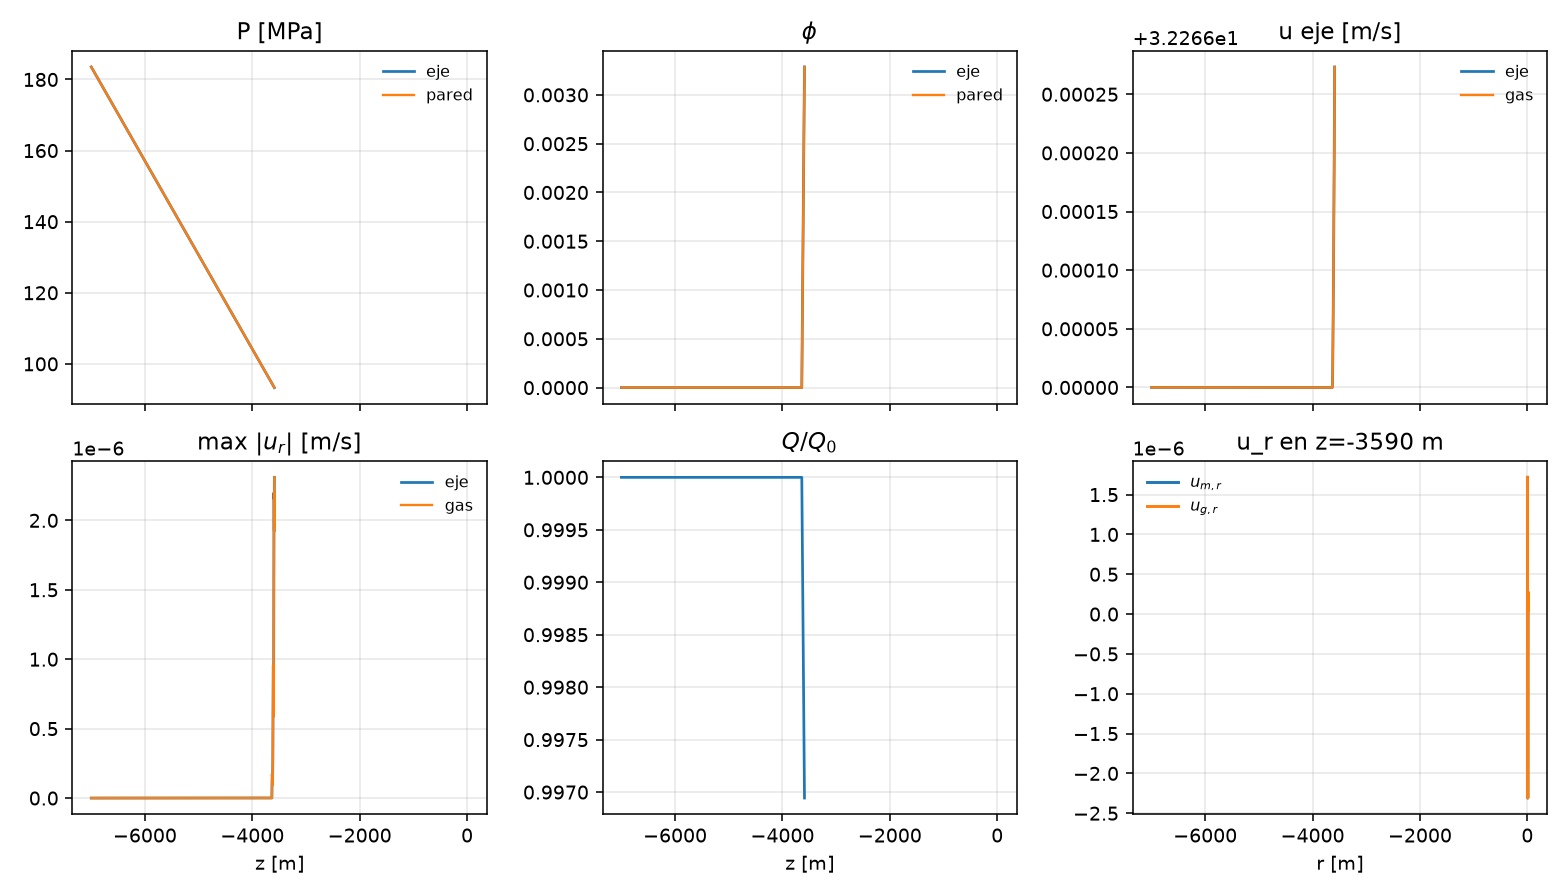
\includegraphics[width=\textwidth]{figuras_variantes/ur_fd.png}
\caption{Marcha en diferencias finitas con las dos componentes
radiales. Hasta la saturación $u_r=0$ y $P$ es la de Poiseuille.
Después las dos fases siguen trabadas y $|u_r|$ permanece
despreciable mientras $\varphi$ es casi uniforme.}
\label{fig:ur-fd}
\end{figure}

\section{Conducto tridimensional}
\label{sec:3d}

El conducto es el cilindro $0\le r\le R$, $0\le\theta<2\pi$,
$H\le z\le 0$, con $t\ge 0$. Las incógnitas dependen de
$(r,\theta,z,t)$. Cada fase tiene tres velocidades. La vertical
de las secciones anteriores es aquí la componente $z$:
$u_{m,z}$ y $u_{g,z}$. El eje-simétrico de la sección~\ref{sec:2d}
es este sistema con
\[
\frac{\p}{\p\theta}=0,
\qquad
u_{m,\theta}=u_{g,\theta}=0,
\qquad
\frac{\p}{\p t}=0.
\]

\subsection{Masa}

\paragraph{Variables.}
$\varphi$ y las dos velocidades
$\mathbf{u}_m=(u_{m,r},u_{m,\theta},u_{m,z})$,
$\mathbf{u}_g=(u_{g,r},u_{g,\theta},u_{g,z})$.
Entran $\rho_g(P)$ y $\Gamma$.

\begin{align}
\label{eq:masa-3d}
\frac{\p}{\p t}\bigl[\rho_m(1-\varphi)\bigr]
+\nabla\cdot\bigl[\rho_m(1-\varphi)\,\mathbf{u}_m\bigr]
&=-\Gamma,
\\
\frac{\p}{\p t}\bigl[\rho_g\,\varphi\bigr]
+\nabla\cdot\bigl[\rho_g\,\varphi\,\mathbf{u}_g\bigr]
&=\Gamma.
\end{align}
En cilíndricas el divergente de un flujo $\mathbf{f}$ es
\begin{equation}
\label{eq:div-cil}
\nabla\cdot\mathbf{f}
=\frac{1}{r}\frac{\p}{\p r}(r f_r)
+\frac{1}{r}\frac{\p f_\theta}{\p\theta}
+\frac{\p f_z}{\p z}.
\end{equation}
El término nuevo respecto del eje-simétrico es
$(1/r)\,\p f_\theta/\p\theta$. El caudal que cruza una sección es
\begin{equation}
\label{eq:Q-3d}
Q(z,t)
=\int_0^{2\pi}\!\int_0^R
\bigl[
\rho_m(1-\varphi)\,u_{m,z}
+\rho_g\,\varphi\,u_{g,z}
\bigr]\,r\,\dd r\,\dd\theta.
\end{equation}
Integrar \eqref{eq:masa-3d} en el disco deja
$\p_t$ de la masa contenida en la rebanada más $\p_z Q$. El flujo
angular se cancela al cerrar $\theta$ en $2\pi$, y el flujo radial
se anula en $r=R$ porque la pared es impermeable.

\subsection{Momento}

\paragraph{Variables.}
$P(r,\theta,z,t)$ y las seis velocidades. Entran $\varphi$, $\mu$,
$\mu_g$ y el arrastre $\mathbf{F}_{mg}$, paralelo al
deslizamiento $\mathbf{u}_g-\mathbf{u}_m$.

La derivada material de la fase fundida es
\begin{equation}
\label{eq:Dt}
\frac{D_m}{Dt}
=\frac{\p}{\p t}
+u_{m,r}\frac{\p}{\p r}
+\frac{u_{m,\theta}}{r}\frac{\p}{\p\theta}
+u_{m,z}\frac{\p}{\p z},
\end{equation}
y $D_g/Dt$ es la misma fórmula con las velocidades del gas. El
viscoseo es el de \eqref{eq:mom-mz}, con la derivada angular
agregada. Sobre una componente $u$,
\begin{equation}
\label{eq:L3}
\begin{aligned}
L[\mu,\varphi]\,u
&=
\frac{1}{r}\frac{\p}{\p r}\Biggl(
r\,\mu(1-\varphi)\frac{\p u}{\p r}
\Biggr)
+\frac{1}{r^2}\frac{\p}{\p\theta}\Biggl(
\mu(1-\varphi)\frac{\p u}{\p\theta}
\Biggr)
\\
&\quad
+\frac{\p}{\p z}\Biggl(
\mu(1-\varphi)\frac{\p u}{\p z}
\Biggr).
\end{aligned}
\end{equation}
En el gas se cambia $\mu(1-\varphi)$ por $\mu_g\varphi$.

En $z$, con $\mathbf{g}$ hacia abajo,
\begin{equation}
\label{eq:mom-3d-z}
\begin{aligned}
\rho_m(1-\varphi)\,\frac{D_m u_{m,z}}{Dt}
&=
-(1-\varphi)\frac{\p P}{\p z}
-\rho_m(1-\varphi)\,g
+F_{mg,z}
+L[\mu,\varphi]\,u_{m,z},
\\[0.4em]
\rho_g\,\varphi\,\frac{D_g u_{g,z}}{Dt}
&=
-\varphi\frac{\p P}{\p z}
-\rho_g\,\varphi\,g
-F_{mg,z}
+L[\mu_g,\varphi]\,u_{g,z}.
\end{aligned}
\end{equation}
En $r$ aparece la aceleración centrífuga $u_\theta^2/r$, y en
$\theta$ el término $u_r u_\theta/r$. Para el fundido,
\begin{align}
\label{eq:mom-3d-r}
\rho_m(1-\varphi)\Biggl(
\frac{D_m u_{m,r}}{Dt}-\frac{u_{m,\theta}^2}{r}
\Biggr)
&=
-(1-\varphi)\frac{\p P}{\p r}
+F_{mg,r}
+L[\mu,\varphi]\,u_{m,r},
\\
\label{eq:mom-3d-th}
\rho_m(1-\varphi)\Biggl(
\frac{D_m u_{m,\theta}}{Dt}+\frac{u_{m,r}\,u_{m,\theta}}{r}
\Biggr)
&=
-(1-\varphi)\frac{1}{r}\frac{\p P}{\p\theta}
+F_{mg,\theta}
+L[\mu,\varphi]\,u_{m,\theta}.
\end{align}
El gas repite \eqref{eq:mom-3d-r}--\eqref{eq:mom-3d-th} con
$\rho_g\varphi$, $D_g$, el signo opuesto de $\mathbf{F}_{mg}$ y
$L[\mu_g,\varphi]$. La ecuación de $P$ es este sistema: las tres
componentes de $\nabla P$ quedan despejadas al pasar el viscoseo
al otro lado, igual que en \eqref{eq:P-2d}. Con
$\p/\p\theta=0$ y $u_\theta=0$, \eqref{eq:mom-3d-z} y
\eqref{eq:mom-3d-r} son el momento de la sección~\ref{sec:2d}, y
\eqref{eq:mom-3d-th} se cumple en la identidad $0=0$.

El arrastre de los regímenes $J_k$ tiene el mismo coeficiente que
\eqref{eq:Fmg1}--\eqref{eq:Fmg4}. La dirección es la del
deslizamiento:
\begin{equation}
\label{eq:Fmg-vec}
\mathbf{F}_{mg}
=\mathcal{C}_k\,(\mathbf{u}_g-\mathbf{u}_m),
\end{equation}
donde $\mathcal{C}_k$ es ese coeficiente dividido por
$(u_g-u_m)$ cuando el deslizamiento es vertical. Sobre el gas
actúa $-\mathbf{F}_{mg}$.

\subsection{Transporte}

\paragraph{Variables.}
$N(r,\theta,z,t)$ y $\xi(r,\theta,z,t)$. Entran $\mathbf{u}_m$,
$\Gamma_N$ y $\Gamma_\xi$, las tasas \eqref{eq:GammaN} y
\eqref{eq:Gammaxi}.

\begin{align}
\label{eq:Nxi-3d}
\frac{\p N}{\p t}+\mathbf{u}_m\cdot\nabla N
&=\Gamma_N,
\\
\frac{\p\xi}{\p t}+\mathbf{u}_m\cdot\nabla\xi
&=\Gamma_\xi.
\end{align}
El producto $\mathbf{u}_m\cdot\nabla$ es $D_m/Dt$ sin la
derivada $\p/\p t$. La exsolución sigue siendo el flujo de masa
por el gradiente de Henry,
\begin{equation}
\label{eq:Gamma-3d}
\Gamma=\mathbf{j}\cdot\nabla n,
\qquad
\mathbf{j}
=\rho_m(1-\varphi)\,\mathbf{u}_m
+\rho_g\,\varphi\,\mathbf{u}_g,
\end{equation}
con $\nabla n=(\p n/\p P)\,\nabla P+(\p n/\p\xi)\,\nabla\xi$.
Ahora $\nabla P$ tiene componente en $\theta$, así que una
variación angular de la presión exsuelve agua aunque $P$ no
cambie con $z$.

\subsection{Condiciones}

En el eje la velocidad cartesiana es un solo vector, así que
\begin{equation}
\label{eq:eje-3d}
u_{m,r}=u_{g,r}=u_{m,\theta}=u_{g,\theta}=0
\quad\text{en }r=0,
\end{equation}
y $\p P/\p r=\p\varphi/\p r=\p N/\p r=\p\xi/\p r=0$. En la pared
el fundido no desliza y ninguna fase la cruza,
\begin{equation}
\label{eq:pared-3d}
\mathbf{u}_m=\mathbf{0},
\qquad
u_{g,r}=0
\quad\text{en }r=R.
\end{equation}
Las componentes tangenciales del gas quedan libres: el roce con
la pared es la versión angular de \eqref{eq:Fmw}. En $\theta$
todo campo cumple $f(\theta+2\pi)=f(\theta)$.

En la base,
$P(r,\theta,H,t)=P_{\mathrm{lit}}+\Delta P(t)$,
$\xi=\xi_0$ y $N=N_0$. En la boca vale una condición, la de
\eqref{eq:boca-t}, ahora en cada $(r,\theta)$:
$P=P_{\mathrm{atm}}$ o $u_{g,z}=c_s$. El dato inicial es una
columna entera
$(P,\varphi,N,\xi,\mathbf{u}_m,\mathbf{u}_g)$ en $t=0$. La
columna eje-simétrica, repetida en $\theta$ con
$u_\theta=0$, es un dato compatible con las marchas de esta
nota. Estas ecuaciones no están integradas: las marchas que sí
corren son las de las secciones anteriores.

\section{Tramo sin burbujas}
\label{sec:sinbub}

Mientras el agua sigue disuelta,
\begin{equation}
\label{eq:sinbub}
\varphi\equiv 0,\qquad \Gamma\equiv 0,\qquad F_{mg}\equiv 0,
\qquad H\le z\le z_{\mathrm{sat}}.
\end{equation}
La masa y el momento del gas quedan en la identidad $0=0$. En este
tramo $u_g$ no entra.

\paragraph{Variables.}
$u(r,z)$ y $P(z)$. Entran $\rho_m(P)$, $\mu$ y $K$.

La masa del fundido en cada radio y el momento vertical son
\begin{align}
\label{eq:masa-sb}
\frac{\p}{\p z}(\rho_m u)&=0,
\\
\label{eq:mom-sb}
\rho_m u\frac{\p u}{\p z}
&=-\frac{\p P}{\p z}-\rho_m g
+\frac{1}{r}\frac{\p}{\p r}\Biggl(r\mu\frac{\p u}{\p r}\Biggr)
+\frac{\p}{\p z}\Biggl(\mu\frac{\p u}{\p z}\Biggr).
\end{align}
Con velocidad radial nula, la componente radial del momento da
$\p P/\p r=0$, luego $P=P(z)$. Los bordes son
\begin{equation}
\label{eq:bc-sb}
\frac{\p u}{\p r}(0,z)=0,
\qquad
u(R,z)=0,
\qquad
P(H)=P_{\mathrm{lit}}+\Delta P.
\end{equation}
Se toman tres cierres, los mismos de la recta algebraica
unidimensional: $\mu$ constante en $r$ y en $z$; módulo de
compresibilidad $K$ constante, $\dd P=K\,\dd\rho_m/\rho_m$; perfil
ya desarrollado, de la forma parabólica \eqref{eq:parabola}, en todo
$H\le z\le z_{\mathrm{sat}}$.

Como $\rho_m=\rho_m(P(z))$, integrar \eqref{eq:masa-sb} deja un
caudal por unidad de área distinto en cada radio y constante en $z$:
\begin{equation}
\label{eq:q-r}
\rho_m(z)\,u(r,z)=q(r),
\qquad
\frac{\p u}{\p z}=-\frac{u}{\rho_m}\frac{\dd\rho_m}{\dd z}.
\end{equation}
Con $K$ constante, $\dd\rho_m/\dd z=(\rho_m/K)\,\dd P/\dd z$. Se
define $c^2=K/\rho_m$. La inercia de \eqref{eq:mom-sb} queda
\begin{equation}
\label{eq:inercia}
\rho_m u\frac{\p u}{\p z}
=-\frac{u(r,z)^2}{c^2}\frac{\dd P}{\dd z}.
\end{equation}
Sustituida en el momento y agrupando $\dd P/\dd z$,
\begin{equation}
\label{eq:puntual}
\frac{\dd P}{\dd z}\Biggl(1-\frac{u(r,z)^2}{c^2}\Biggr)
=-\rho_m g
+\frac{1}{r}\frac{\p}{\p r}\Biggl(r\mu\frac{\p u}{\p r}\Biggr)
+\frac{\p}{\p z}\Biggl(\mu\frac{\p u}{\p z}\Biggr).
\end{equation}
El factor $1-u^2/c^2$ depende de $r$. Una sola $P(z)$ se obtiene
promediando \eqref{eq:puntual} en la sección,
\begin{equation}
\label{eq:prom}
\langle f\rangle=\frac{2}{R^2}\int_0^R f(r)\,r\,\dd r.
\end{equation}
Con $\mu$ constante el promedio del laplaciano radial es el esfuerzo
en la pared:
\begin{equation}
\label{eq:Lr-pared}
\Biggl\langle
\frac{1}{r}\frac{\p}{\p r}\Biggl(r\mu\frac{\p u}{\p r}\Biggr)
\Biggr\rangle
=\frac{2\mu}{R}\frac{\p u}{\p r}\bigg|_{r=R}.
\end{equation}
El perfil que cumple \eqref{eq:bc-sb} es
\begin{equation}
\label{eq:parabola}
u(r,z)=u_c(z)\Biggl(1-\frac{r^2}{R^2}\Biggr)
=2\bar u(z)\Biggl(1-\frac{r^2}{R^2}\Biggr),
\end{equation}
porque la media de la parábola es $\bar u=u_c/2$. Entonces
$\p u/\p r|_{r=R}=-4\bar u/R$ y
\begin{equation}
\label{eq:roce}
\Biggl\langle
\frac{1}{r}\frac{\p}{\p r}\Biggl(r\mu\frac{\p u}{\p r}\Biggr)
\Biggr\rangle
=-\frac{8\mu\bar u}{R^2}.
\end{equation}
El caudal medio cumple $\bar u=\bar q/\rho_m$. La forma se conserva;
la amplitud cambia cuando cambia $\rho_m$. El promedio del cuadrado
sobre \eqref{eq:parabola} es
\begin{equation}
\label{eq:u2}
\langle u^2\rangle=\frac43\bar u^2.
\end{equation}
El factor $4/3$ es el peso del centro, que va al doble de la media.

El esfuerzo axial que produce esta compresión, con $\mu$ y $K$
constantes, es
\begin{equation}
\label{eq:axial}
\frac{\p}{\p z}\Biggl(\mu\frac{\p u}{\p z}\Biggr)
=\mu\frac{u}{K^2}\Biggl(\frac{\dd P}{\dd z}\Biggr)^2
-\mu\frac{u}{K}\frac{\dd^2 P}{\dd z^2}.
\end{equation}
Frente al roce \eqref{eq:roce}, el primer término está en la razón
$R^2|\dd P/\dd z|^2/(8K^2)$. Con
$|\dd P/\dd z|\sim 3\times 10^{4}\Pam$, $K=1{,}5\times 10^{10}\,\mathrm{Pa}$
y $R=16\,\mathrm{m}$, esa razón es del orden de $10^{-10}$. Se retira
\eqref{eq:axial} del promedio.

\begin{proposicion}
Bajo \eqref{eq:sinbub}, \eqref{eq:bc-sb} y los tres cierres de esta
sección,
\begin{equation}
\label{eq:dpdz}
\frac{\dd P}{\dd z}
=\frac{-\rho_m g-8\mu\bar u/R^2}{1-\frac43\bar u^2/c^2},
\qquad
c^2=\frac{K}{\rho_m},
\qquad
\bar u=\frac{\bar q}{\rho_m}.
\end{equation}
\end{proposicion}

El numerador es el peso más el roce de pared de la parábola. El
denominador es la inercia de la compresión después de promediar
$u(r)^2$. Si el perfil fuera plano, $\langle u^2\rangle=\bar u^2$ y
el denominador quedaría $1-\bar u^2/c^2$, que es el factor de la
recta algebraica unidimensional.

Con $\rho_m$, $\mu$ y $\bar u=\vin$ congelados y $K=15\,\mathrm{GPa}$,
\eqref{eq:dpdz} es constante y
$P(z)=P(H)+(\dd P/\dd z)\,(z-H)$ hasta
\begin{equation}
\label{eq:Psat}
P(z_{\mathrm{sat}})=P_{\mathrm{sat}}=\bigl(c_0/C_1\bigr)^{1/\beta}.
\end{equation}
En la base de Calbuco, con $\bar u=18{,}3\ms$, $c=2468\ms$ y
$\rho_m=2463\,\mathrm{kg\,m^{-3}}$, se tiene
$\bar u^2/c^2=5{,}5\times 10^{-5}$. El denominador de \eqref{eq:dpdz}
vale $1-7{,}3\times 10^{-5}$. Sobre una pendiente de
$2{,}677\times 10^{4}\Pam$, el divisor corrige unos $2\Pam$.

La parábola describe el tramo ya desarrollado. Un tapón uniforme en
la base, $u=\vin$ para $r<R$ y $u(R)=0$, cumple el borde y tiene
laplaciano nulo en el interior. La longitud en que el viscoseo
radial lo acomoda a \eqref{eq:parabola} es
$L\sim\rho_m\vin R^2/\mu$, del orden de $2{,}5\,\mathrm{km}$ con los
números de la base. En Calbuco, $z_{\mathrm{sat}}$ cae cerca de
$-3{,}7\,\mathrm{km}$. La fórmula \eqref{eq:dpdz} cubre desde ese
acomodo hasta la saturación.

\subsection{Diferencias finitas hasta la saturación}

El tramo se integró en diferencias finitas sin imponer
$u_{m,r}=0$ dentro del conducto. En cada paso el residuo de la masa,
del momento axial y del momento radial se lleva a cero.
$\rho_m=\rho_m(H)\exp\bigl((P-P(H))/K\bigr)$ con $K=15\,\mathrm{GPa}$.
Los datos de borde son $u_{m,r}=0$ en el eje, en la pared y en la
base, $u_m(R)=0$, y en $z=H$ la parábola con
$\bar u=16{,}133\,\mathrm{m/s}$ y $P=P_{\mathrm{lit}}+\Delta P$.
Hay $17$ nodos en $r$ y pasos de $40\,\mathrm{m}$.

La marcha corta en $z=-3635\,\mathrm{m}$, cuando
$P=P_{\mathrm{sat}}=94{,}72\,\mathrm{MPa}$. El caudal de masa se
conserva al nivel de $10^{-7}$ relativo. $\rho_m$ en el eje pasa de
$2463{,}2$ a $2448{,}7\,\mathrm{kg\,m^{-3}}$ y $\bar u$ de $16{,}07$
a $16{,}17\,\mathrm{m/s}$: el producto $\rho_m\bar u$ queda fijo.
$|u_{m,r}|$ baja de $10^{-4}\,\mathrm{m/s}$ en el primer paso a
menos de $10^{-8}\,\mathrm{m/s}$ en el resto del tramo, y $P$ no
depende de $r$. $\partial P/\partial z$ en el eje va de
$-2{,}645\times 10^{4}$ a $-2{,}633\times 10^{4}\,\mathrm{Pa/m}$.
La fórmula \eqref{eq:dpdz}, evaluada con el $\rho_m$ y el $\bar u$
de cada altura, cae a $10\,\mathrm{Pa/m}$ de ese valor.

\begin{figure}[ht]
\centering
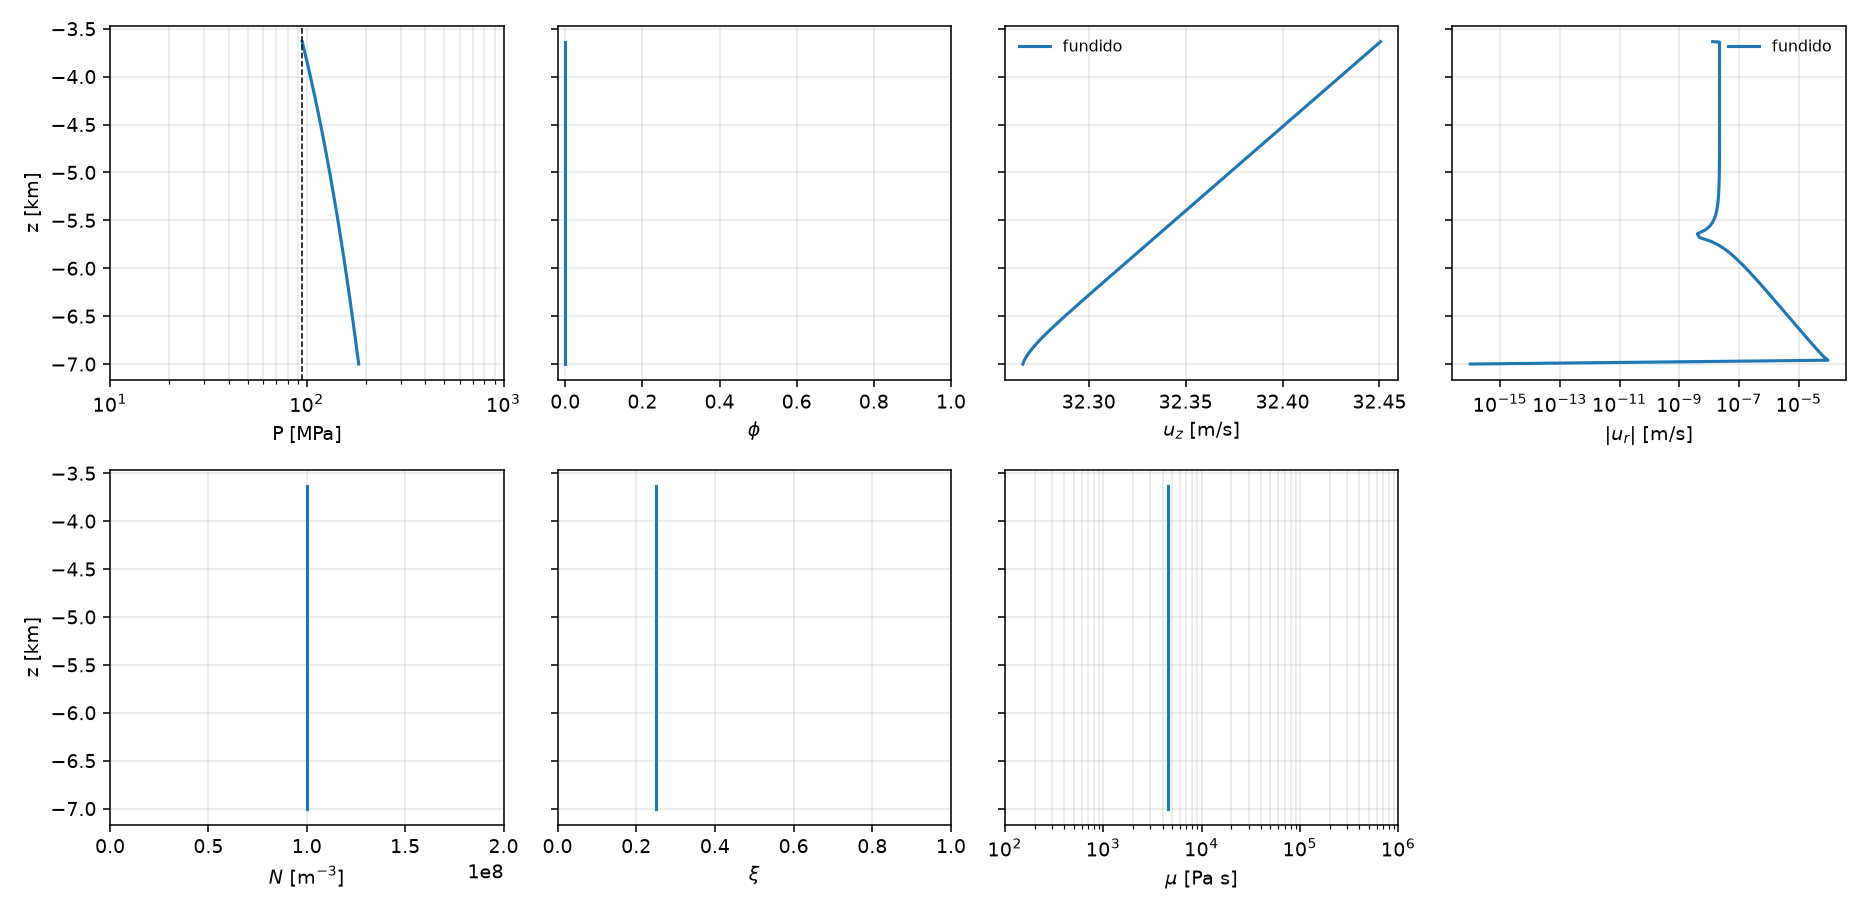
\includegraphics[width=\textwidth]{figuras_variantes/sinbub_fd.png}
\caption{Tramo sin exsolución. La profundidad está en el eje
vertical. $P$, $|u_r|$ y $\mu$ van en escala logarítmica
horizontal. $\varphi=0$, $N=10^{8}\,\mathrm{m^{-3}}$ y
$\xi=\xi_0=0{,}25$. El gas no entra: no hay curva de $u_g$.}
\label{fig:sinbub-fd}
\end{figure}

\begin{figure}[ht]
\centering
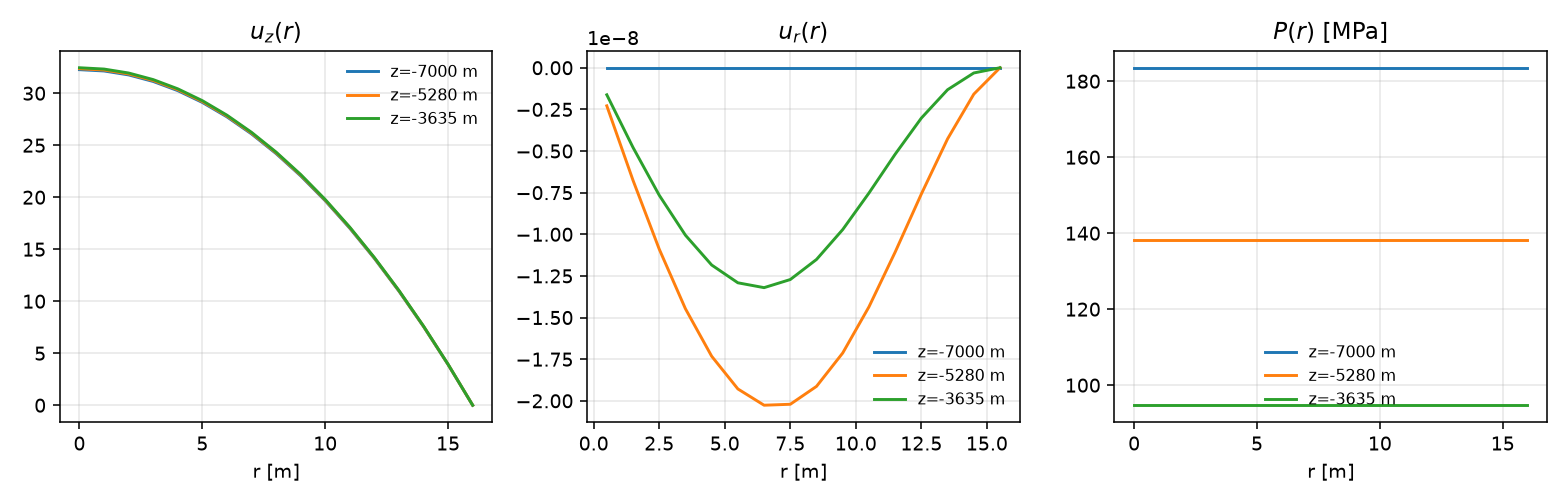
\includegraphics[width=\textwidth]{figuras_variantes/sinbub_fd_perfiles.png}
\caption{Perfiles en la base, a media altura y al llegar a
$P_{\mathrm{sat}}$. $u_r$ queda en el ruido de la malla y $P$ es
uniforme en $r$.}
\label{fig:sinbub-perfiles}
\end{figure}

\subsection{El metro donde empieza la exsolución}

En $z_{\mathrm{sat}}$ se tiene $n=0$ y $\varphi=0$, y la velocidad
del gas, escrita como caudal de gas sobre $\varphi\rho_g$, queda
indeterminada. El estado inicial de la marcha se arma un metro más
arriba. Si la saturación cae a menos de un metro de la boca, ese
desplazamiento es $-z_{\mathrm{sat}}/10$. Con $\varepsilon=1\,\mathrm{m}$,
\begin{equation}
\label{eq:zad}
z_{\mathrm{ad}}=z_{\mathrm{sat}}+\varepsilon,
\qquad
P_{\mathrm{ad}}=P_{\mathrm{sat}}+\frac{\dd P}{\dd z}\,\varepsilon.
\end{equation}
Como $\dd P/\dd z<0$, se tiene $P_{\mathrm{ad}}<P_{\mathrm{sat}}$ y
Henry ya suelta agua. Con $\xi$ todavía igual a $\xi_0$,
\begin{equation}
\label{eq:nad}
n_{\mathrm{ad}}
=\frac{(1-\xi_0)c_0-C_1 P_{\mathrm{ad}}^{\beta}}{1-C_1 P_{\mathrm{ad}}^{\beta}}.
\end{equation}
$P_{\mathrm{ad}}$ y $\xi_0$ no dependen de $r$, así que
$n_{\mathrm{ad}}$ es constante en la sección.
$\rho_{g,\mathrm{ad}}=P_{\mathrm{ad}}/(\Rv T)$.

\begin{proposicion}
En $z_{\mathrm{ad}}$, con el caudal $q(r)$ heredado del tramo sin
burbujas,
\begin{equation}
\label{eq:phi-ad}
\varphi_{\mathrm{ad}}
=\Biggl(
1+\frac{P_{\mathrm{ad}}}{n_{\mathrm{ad}}\Rv T}
\frac{1-n_{\mathrm{ad}}}{\rho_m}
\Biggr)^{-1},
\end{equation}
\begin{equation}
\label{eq:u-ad}
u_m(r)=u_g(r)
=\frac{q(r)\,(1-n_{\mathrm{ad}})}{(1-\varphi_{\mathrm{ad}})\,\rho_m}
=2\bar u_{\mathrm{ad}}\Biggl(1-\frac{r^2}{R^2}\Biggr),
\end{equation}
\begin{equation}
\label{eq:uad-media}
\bar u_{\mathrm{ad}}
=\frac{\bar q\,(1-n_{\mathrm{ad}})}{(1-\varphi_{\mathrm{ad}})\,\rho_m}
=\frac{\bar q\,n_{\mathrm{ad}}}{\varphi_{\mathrm{ad}}\,\rho_{g,\mathrm{ad}}},
\qquad
q(r)=2\bar q\Biggl(1-\frac{r^2}{R^2}\Biggr).
\end{equation}
En la pared, $q(R)=0$. $N$ y $\xi$ siguen en $N_0$ y $\xi_0$.
\end{proposicion}

La suma de las dos masas conserva $q(r)$. Se parte con
\eqref{eq:nad}: $\rho_g\varphi u_g=n_{\mathrm{ad}}q(r)$ y
$\rho_m(1-\varphi)u_m=(1-n_{\mathrm{ad}})q(r)$. El cociente de
volúmenes es $\varphi_{\mathrm{ad}}$. De esa definición las dos
velocidades coinciden, y con la parábola de $q(r)$ se obtiene
\eqref{eq:u-ad}. $\varphi_{\mathrm{ad}}$ no depende de $r$. El
deslizamiento $u_g-u_m$ aparece al integrar el momento desde
$z_{\mathrm{ad}}$.

\section{Capilar en cada radio}

El estado de referencia de un tiro es el de
\eqref{eq:Ca-ast}: $P^\ast$ deja la fracción de Henry a menos de
$0{,}002$ de $\varphi^\ast=0{,}2$, con $\xi=\xi_0$. En ese estado
$n$ y $\varphi$ no dependen de $r$. La velocidad media obedece la
masa del fundido,
\begin{equation}
\label{eq:umed}
\bar u=\vin\frac{1-n}{1-\varphi},
\end{equation}
y el perfil es la parábola \eqref{eq:parabola}. Entonces
\begin{equation}
\label{eq:dudz}
\frac{\dd\bar u}{\dd z}
=\vin
\frac{
-\dfrac{\dd n}{\dd P}(1-\varphi)+(1-n)\dfrac{\dd\varphi}{\dd P}
}{(1-\varphi)^2}
\frac{\dd P}{\dd z},
\end{equation}
con las derivadas de Henry y del volumen \eqref{eq:phi-ad} en
$P^\ast$, y con $\dd P/\dd z$ la pendiente de Poiseuille de ese
estado. Sobre la parábola,
\begin{equation}
\label{eq:du}
\frac{\p u}{\p z}
=2\frac{\dd\bar u}{\dd z}\Biggl(1-\frac{r^2}{R^2}\Biggr),
\qquad
\frac{\p u}{\p r}=-\frac{4\bar u\, r}{R^2}.
\end{equation}
En el eje, $\p u/\p r=0$ y $\p u/\p z=2\,\dd\bar u/\dd z$. En la
pared, $\p u/\p z=0$ y $\p u/\p r=-4\bar u/R$.

\paragraph{Variables.}
$\mathrm{Ca}(r)$. Entran $\dot\varepsilon(r)$, $\mu(r)$ y $r_b$.
El radio de burbuja es \eqref{eq:rb} con $\varphi^\ast$ y $N_0$, y
no depende de $r$.

La tasa que entra al capilar en el radio $r$ es
\begin{equation}
\label{eq:eps}
\dot\varepsilon(r)
=\frac12\Biggl(
\biggl|\frac{\p u}{\p z}\biggr|
+\biggl|\frac{\p u}{\p r}\biggr|
\Biggr).
\end{equation}
Con \eqref{eq:du}, $\dot\varepsilon(0)=|\dd\bar u/\dd z|$ y
$\dot\varepsilon(R)=2\bar u/R$. $\mu(r)$ se evalúa en $P^\ast$, con
el agua disuelta $C_1 P^{\beta}$, al corte $|\p u/\p r|$. Entonces
\begin{equation}
\label{eq:Ca-r}
\mathrm{Ca}(r)=\frac{\dot\varepsilon(r)\,\mu(r)\,r_b}{0{,}3},
\end{equation}
y $\varphi_{\mathrm{crit}}(r)$, $\varphi_1(r)$, $\varphi_2(r)$ son
\eqref{eq:umbrales-Ca} evaluadas en $\mathrm{Ca}(r)$. Se calculan
una vez por tiro, junto con $N_0$. En el eje el capilar siente la
extensión de la media. En la pared siente el corte $4\bar u/R$.

\section{Marcha antes de fragmentar}
\label{sec:marcha}

Una llamada con $\vin$ fijo integra una columna. El tiro es el lazo
exterior: se repite la integración hasta que la boca cumple
\begin{equation}
\label{eq:boca}
P(0)=P_{\mathrm{atm}}
\quad\text{o}\quad
\max_r u_g(r,0)\approx c_s=\sqrt{\Rv T}.
\end{equation}

La malla radial es $r_i=i\Delta r$, $r_I=R$. En $z$ el paso $h_j$
es variable y las derivadas van hacia atrás,
\begin{equation}
\label{eq:Dz}
(D_z^- f)_{i,j}=\frac{f_{i,j}-f_{i,j-1}}{h_j}.
\end{equation}
El laplaciano viscoso de la mezcla es la diferencia conservativa
$L_r[\mu,\varphi]u$. En el eje se reemplaza por
$4\mu(1-\varphi)(u_1-u_0)/\Delta r^2$. En la pared,
$u_I=u_g{}_{I}=0$.

\paragraph{Variables del paso.}
$u_{i}(z_j)$ y el escalar $\dd P/\dd z$. Entran $\mu(u)$, $\varphi_i$
y el caudal $Q$.

Mientras $\varphi$ no ha pasado $\varphi_{\mathrm{crit}}$ en toda
la sección, el momento que se discretiza es el de la mezcla, con
una sola velocidad. La viscosidad depende de esa velocidad. El
sistema del paso es no lineal y se resuelve por Picard: en el
iterado $k$ se congelan $\mu^{(k)}=\mu(u^{(k)})$ y
$u^\star=u^{(k)}$, y se resuelve
\begin{equation}
\label{eq:picard}
\begin{aligned}
L_r[\mu^{(k)},\varphi]\,u^{(k+1)}
+\rho_c\frac{u^\star}{h}u^{(k+1)}
&=
-\rho_c g+\frac{\sigma^\star-\sigma_{j-1}}{h}
+\rho_c\frac{u^\star}{h}u_{j-1}
\\
&\quad
-(1-\varphi)\frac{\dd P}{\dd z}.
\end{aligned}
\end{equation}
$L_r$ más el término de inercia en la diagonal es tridiagonal. Cada
iterado lo resuelve el algoritmo de Thomas. $\dd P/\dd z$ es el
único número que hace que el flujo de $\rho_c u^{(k+1)}$ integre
$Q$. La presión del paso nuevo no vuelve a entrar en esa iteración:
si $\varphi$ se actualizara con $P$ dentro del mismo Picard, la
densidad bajaría y $\dd P/\dd z$ se dispararía. El esfuerzo axial
entra congelado, del lado derecho.

Cerrado el iterado, se acepta el paso si un paso de tamaño $h$ y
dos de tamaño $h/2$ difieren poco en $P$ y en $\varphi$. Si no, se
rechaza y se parte $h$. En este tramo
\begin{equation}
\label{eq:cierre-pre}
\varphi_i=\varphi_{\mathrm{Henry}}(P,\xi_i),
\qquad
u_{g,i}=u_i.
\end{equation}
$P=P(z)$. $\xi$ parte de $\xi_0$ en todos los radios. Con
$\tau_c=2\,\mathrm{h}$ el ascenso dura del orden de un minuto, así
que $\xi$ casi no se mueve y $\varphi_i$ sale igual en todos los
nodos. Lo que sí depende de $r$ en esta marcha es $u_m$, y con él
$\mathrm{Ca}$, $\varphi_1$ y $\varphi_{\mathrm{crit}}$.

\section{Después de la fragmentación}
\label{sec:frag}

Cuando $\varphi_i\ge\varphi_{\mathrm{crit}}(r_i)$ en toda la
sección se deja el momento de la mezcla. $N$ y $\xi$ quedan en el
valor del cruce. El caudal $q(r)$ de cada radio es el que trae la
marcha hasta $z_f$,
\begin{equation}
\label{eq:q-f}
q(r)
=\rho_m(1-\varphi_f)\,u_{m,f}
+\rho_g(z_f)\,\varphi_f\,u_{g,f},
\end{equation}
y no se vuelve a modificar. Los cristales quedan en el líquido, así
que el reparto de esa masa entre líquido y gas se evalúa sin $\xi$
en el factor del gas:
\begin{equation}
\label{eq:n-frag}
n(P)
=\Biggl(1+\frac{\rho_g(P)}{\rho_m}\Biggl(\frac{1}{c_g(P)}-1\Biggr)\Biggr)^{-1}.
\end{equation}
El salto de $u_g$ en $z_f$, del orden de $1/(1-\xi_0)=4/3$, es el
paso desde la fórmula de masa con $\xi$ a \eqref{eq:n-frag}.
El arrastre de las corridas de esta sección es
$F_{mg}=C\,\varphi(1-\varphi)(u_g-u_m)|u_g-u_m|$ con
$C=300\,\mathrm{m}^{-1}$.

\subsection{Promedio de sección}

\paragraph{Variables.}
$P(z)$ y $\bar\varphi(z)$. Entran $\bar q$, $n(P)$ y $F_{mg}$
evaluado con las medias.

\begin{equation}
\label{eq:umedias}
\bar u_m=\frac{(1-n)\,\bar q}{\rho_m(1-\bar\varphi)},
\qquad
\bar u_g=\frac{n\,\bar q}{\rho_g\,\bar\varphi},
\end{equation}
\begin{align}
\label{eq:mom-media}
\rho_m\bar u_m\frac{\dd\bar u_m}{\dd z}
+\frac{\dd P}{\dd z}+\rho_m g
-\frac{F_{mg}}{1-\bar\varphi}
&=0,
\\
\rho_g\bar u_g\frac{\dd\bar u_g}{\dd z}
+\frac{\dd P}{\dd z}+\rho_g g
+\frac{F_{mg}}{\bar\varphi}
&=0.
\end{align}
De \eqref{eq:mom-media} salen $\dd P/\dd z$ y $\dd\bar\varphi/\dd z$,
un par para toda la sección. Las velocidades de cada radio se
reconstruyen con el mismo $n$ y con el $q(r)$ de \eqref{eq:q-f}.
El perfil radial que traía Thomas se conserva por encima de $z_f$.
El roce del fundido con la pared no entra en este par: es el mismo
sistema algebraico del régimen fragmentado unidimensional, evaluado
en $\bar\varphi$, $\bar q=Q/(\pi R^2)$ y $\bar\xi$. El incremento
\begin{equation}
\label{eq:dphi}
\varphi_i\leftarrow\varphi_i+h\frac{\dd\bar\varphi}{\dd z}
\end{equation}
es el mismo en todos los radios. Si $\varphi$ era plano en $r$,
sigue plano.

\subsection{La pendiente que pide cada radio}

\paragraph{Variables.}
$\dd P/\dd z$ en cada $r$, con $q(r)$ y $\varphi_f$ fijos.

Si \eqref{eq:mom-media} se escribe en el radio, sin promediar,
$\dd P/\dd z$ deja de ser único. Con $\vin=17{,}021\ms$ la
fragmentación cae en $z_f=-906{,}2\,\mathrm{m}$,
$P_f=12{,}00\MPa$ y $\varphi_f=0{,}702$.

\begin{table}[ht]
\centering
\caption{Caudal congelado y pendiente de presión en $z_f$.
El promedio de la sección pide
$\dd P/\dd z=-5{,}8\times 10^{5}\Pam$.}
\label{tab:dpdz-r}
\begin{tabular}{@{}lrr@{}}
\toprule
radio & $q$ [$\mathrm{kg\,m^{-2}s^{-1}}$]
& $\dd P/\dd z$ [\Pam] \\
\midrule
eje & $9{,}41\times 10^{4}$ & $-3{,}77\times 10^{6}$ \\
medio & $5{,}76\times 10^{4}$ & $-1{,}38\times 10^{6}$ \\
cerca de la pared & $6{,}91\times 10^{3}$ & $-2{,}30\times 10^{4}$ \\
\bottomrule
\end{tabular}
\end{table}

El eje lleva unas catorce veces más masa que la pared. Una sola
$P(z)$ no cumple \eqref{eq:mom-media} en todos los radios a la vez.

\subsection{Presión propia de cada radio}

\paragraph{Variables.}
$P(r,z)$ y $\varphi(r,z)$. En cada radio, $u_m$ y $u_g$ por
\eqref{eq:vel} con el $q(r)$ congelado y $n(P)$ de
\eqref{eq:n-frag}.

\begin{align}
\label{eq:mom-loc}
\rho_m u_m\frac{\dd u_m}{\dd z}
+\frac{\dd P}{\dd z}+\rho_m g
-\frac{F_{mg}}{1-\varphi}
&=0,
\\
\rho_g u_g\frac{\dd u_g}{\dd z}
+\frac{\dd P}{\dd z}+\rho_g g
+\frac{F_{mg}}{\varphi}
&=0.
\end{align}
Integrado en el eje con la fragmentación en $z_f=-906\,\mathrm{m}$
($P_f=12\MPa$, $u_{g,f}=67\ms$, $u_{m,f}=16\ms$), la marcha se
detiene en $z=-905\,\mathrm{m}$. Ahí $P=8{,}59\MPa$,
$u_g=757\ms$, $u_m=65\ms$ y $\varphi=0{,}841$.

\begin{figure}[ht]
\centering
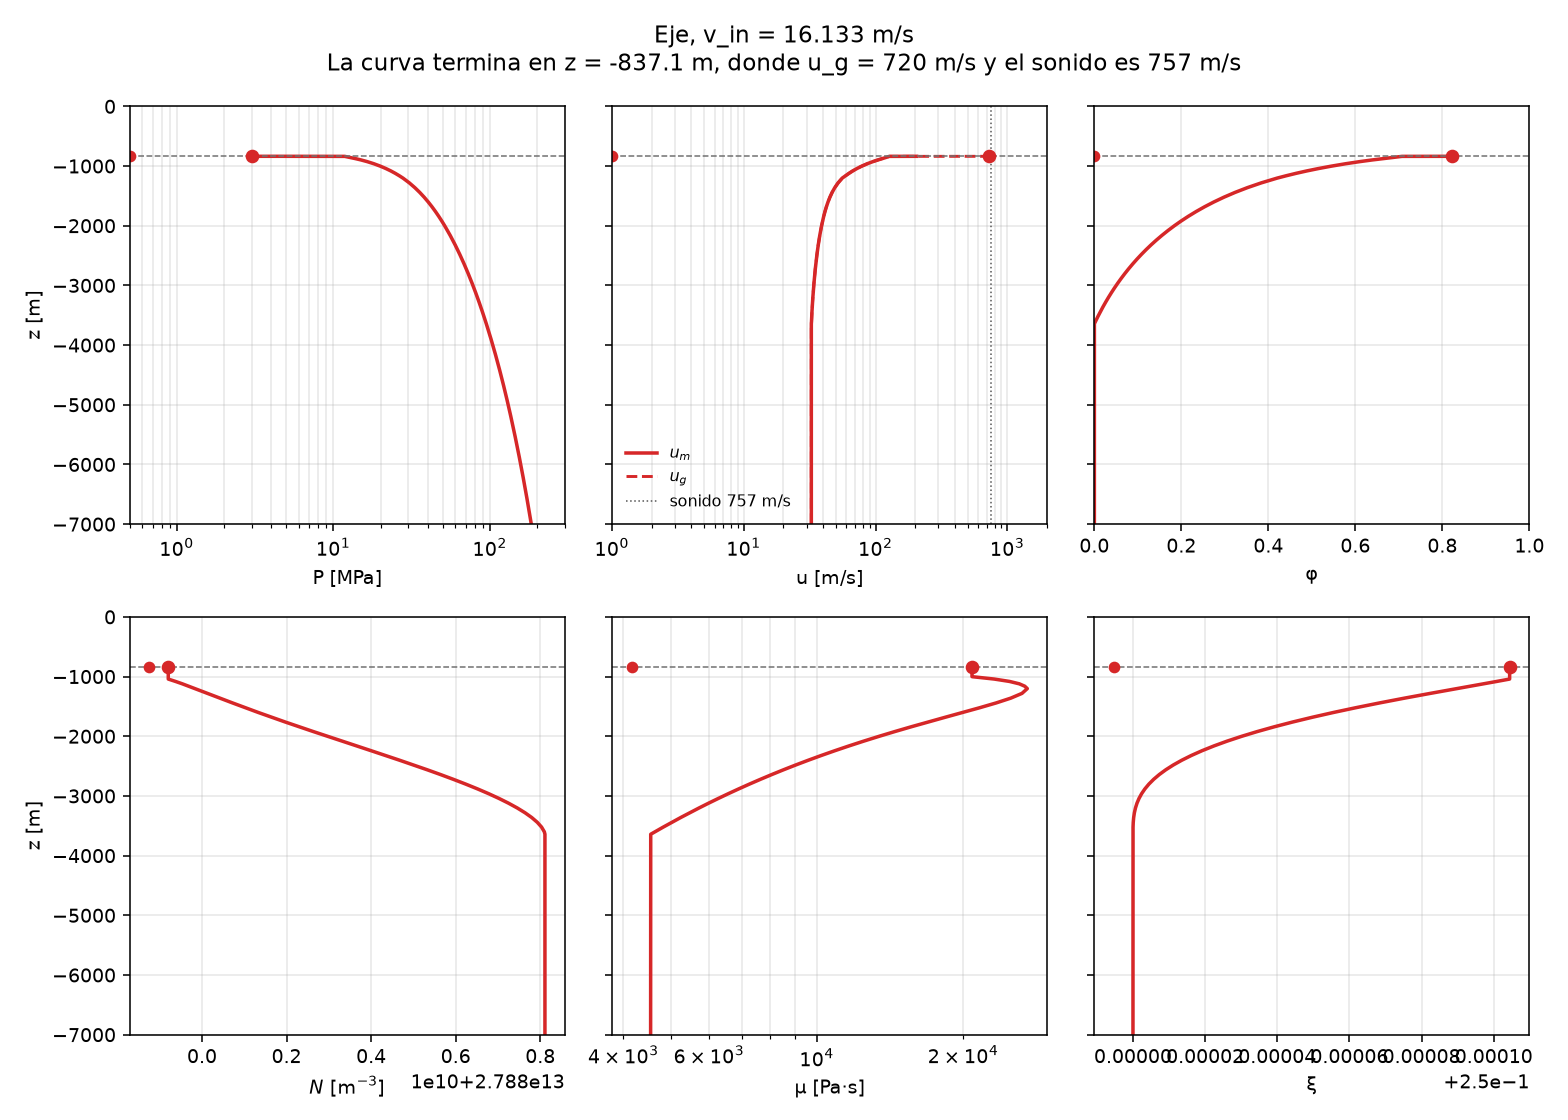
\includegraphics[width=\textwidth]{perfiles-eje.png}
\caption{Eje, sistema \eqref{eq:mom-loc}. La columna se corta en
$z=-905\,\mathrm{m}$, un metro sobre $z_f=-906\,\mathrm{m}$, cuando
$u_g$ llega a $757\ms$.}
\label{fig:eje}
\end{figure}

\subsection{Laplaciano viscoso del gas}

\paragraph{Variables.}
Las de \eqref{eq:mom-loc}, más $L_r$ en el momento del gas. $L_r$
depende de $\mu_g$, $\varphi$ y $\p_r u_g$.

\begin{equation}
\label{eq:Lr-g}
L_r
=\frac{1}{r}\frac{\p}{\p r}\Biggl(
r\,\mu_g\,\varphi\,\frac{\p u_g}{\p r}\Biggr),
\qquad
\mu_g=10^{-5}\,\mathrm{Pa\cdot s}.
\end{equation}
El momento del gas gana el término $-L_r/\varphi$. En
$z_f=-906{,}2\,\mathrm{m}$, con $\vin=17{,}021\ms$, se mide
$|L_r|_{\max}=4{,}6\times 10^{-3}\Pam$. Al lado de
$\dd P/\dd z\sim 10^{6}\Pam$ los perfiles no se mueven: el eje se
corta al hacerse sónico y la pared llega a $z=0$ subsónica.

\begin{figure}[ht]
\centering
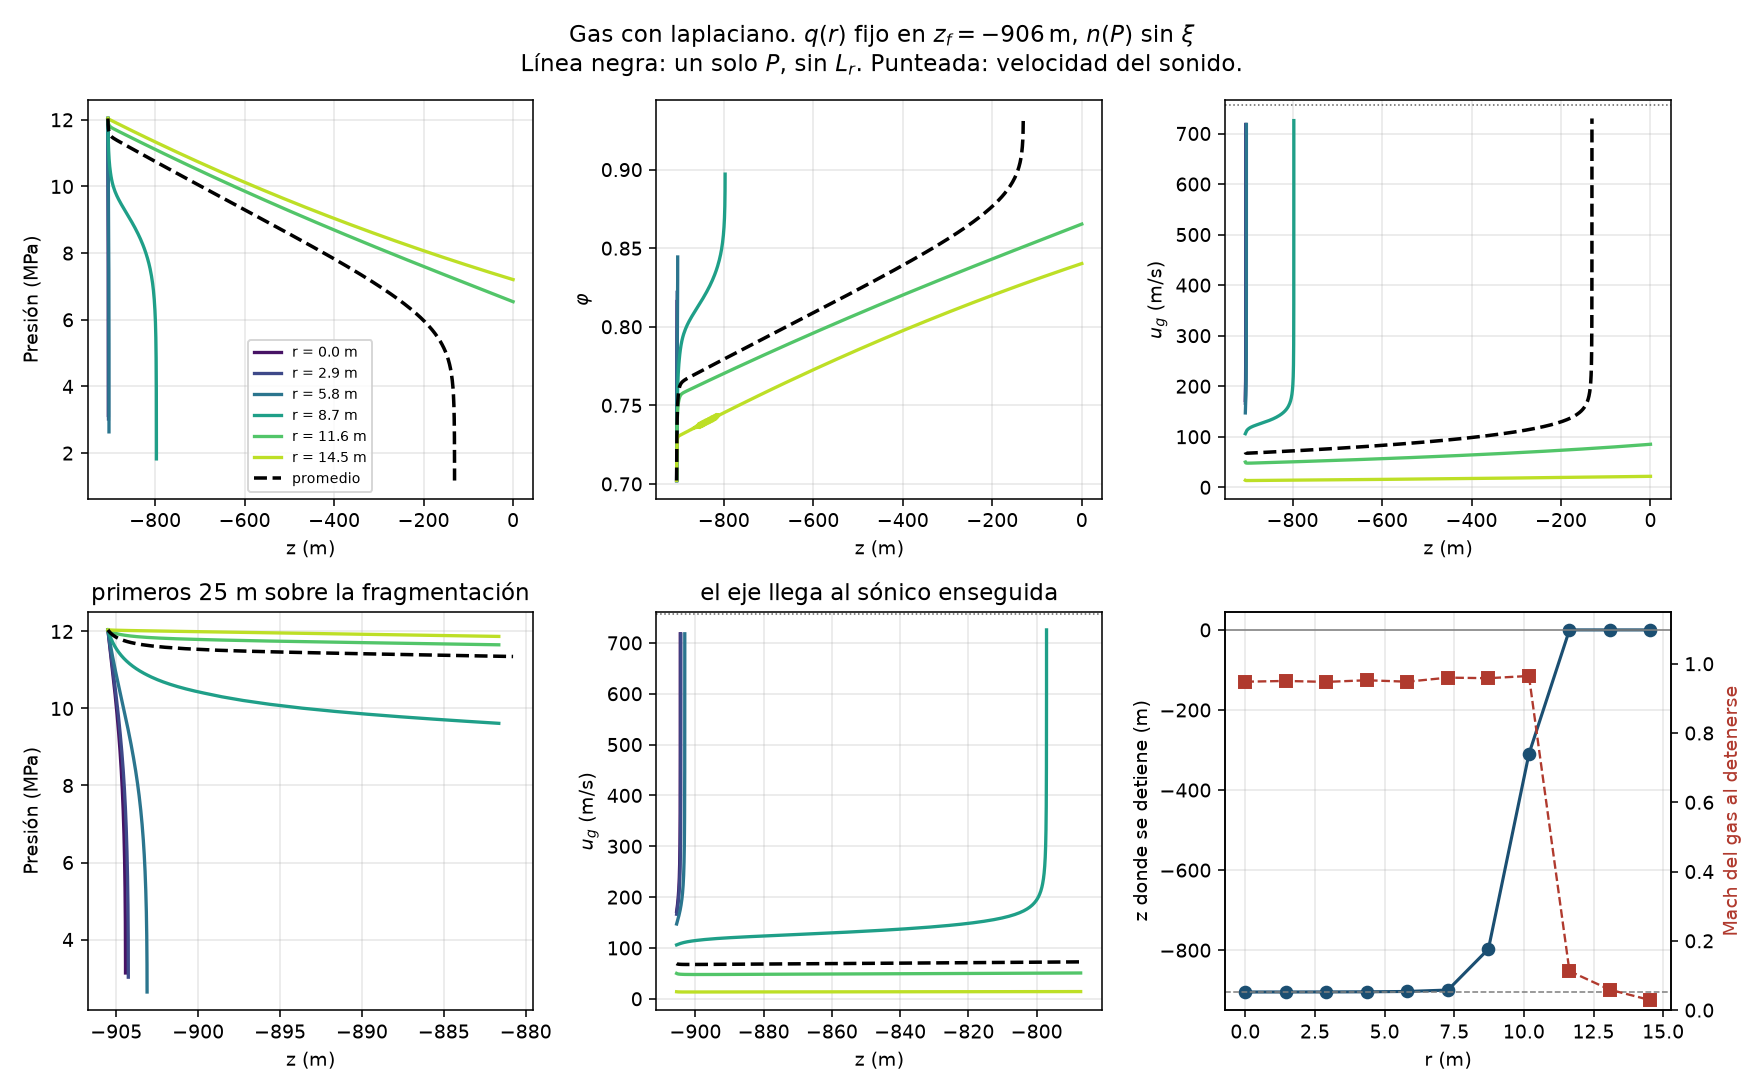
\includegraphics[width=\textwidth]{edp-local-con-laplaciano.png}
\caption{Sistema local con \eqref{eq:Lr-g}.
$|L_r|_{\max}=4{,}6\times 10^{-3}\Pam$ en
$z_f=-906{,}2\,\mathrm{m}$. Arriba, $\varphi$, $P$, $u_m$ y $u_g$
frente a $z-z_f$ en el eje, en un radio medio y en la pared.
Abajo, $q(r)$, $\dd P/\dd z$ y $|L_r|$ en la fragmentación.}
\label{fig:lap}
\end{figure}

\subsection{Tiro de la media}

El tiro sobre \eqref{eq:mom-media} busca el $\vin$ que deja
$\bar u_g$ sónica en la boca. Converge en
$\vin=16{,}133\ms$. La fragmentación queda en
$z_f=-838\,\mathrm{m}$, con $u_{g,f}=51{,}1\ms$. La media llega a
$z=-0{,}44\,\mathrm{m}$ con $P=1{,}11\MPa$ y $\bar u_g=730\ms$.

\begin{figure}[ht]
\centering
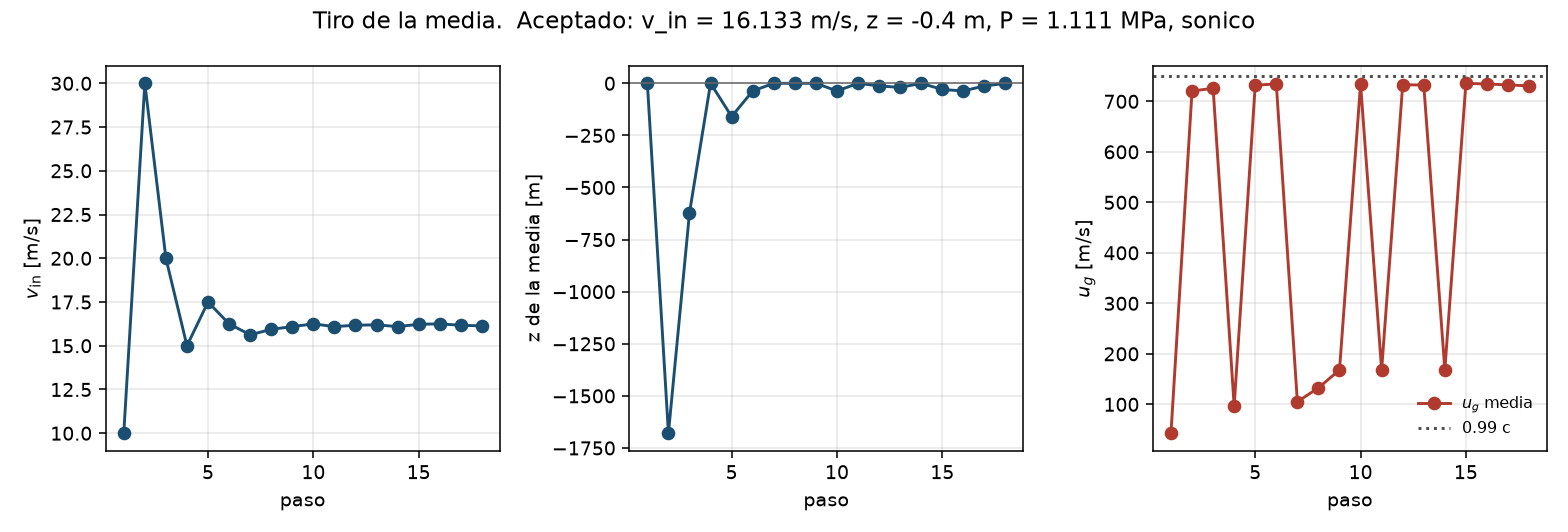
\includegraphics[width=0.72\textwidth]{tiro-vin.png}
\caption{Tiro de $\bar u_g$. $\vin=16{,}133\ms$, boca en
$z=-0{,}44\,\mathrm{m}$ con $P=1{,}11\MPa$ y $\bar u_g=730\ms$.}
\label{fig:tiro}
\end{figure}

Ese $\vin$ fija la sección. El eje, integrado con \eqref{eq:mom-loc}
y su propio $q(0)$, se detiene un metro sobre $z_f$. Con la misma
entrada, el radio $r=13{,}1\,\mathrm{m}$ llega a la boca.

Fragmentación común en $z_f=-838\,\mathrm{m}$, $P_f=10\MPa$,
$u_{g,f}=51\ms$. El eje se detiene en $z=-837\,\mathrm{m}$ con
$P=7{,}15\MPa$, $u_g=757\ms$, $u_m=49\ms$ y $\varphi=0{,}866$.
El radio $r=13{,}1\,\mathrm{m}$ llega a $z=0$ con $P=6{,}95\MPa$,
$u_g=80\ms$, $u_m=5{,}2\ms$ y $\varphi=0{,}871$.

\begin{figure}[ht]
\centering
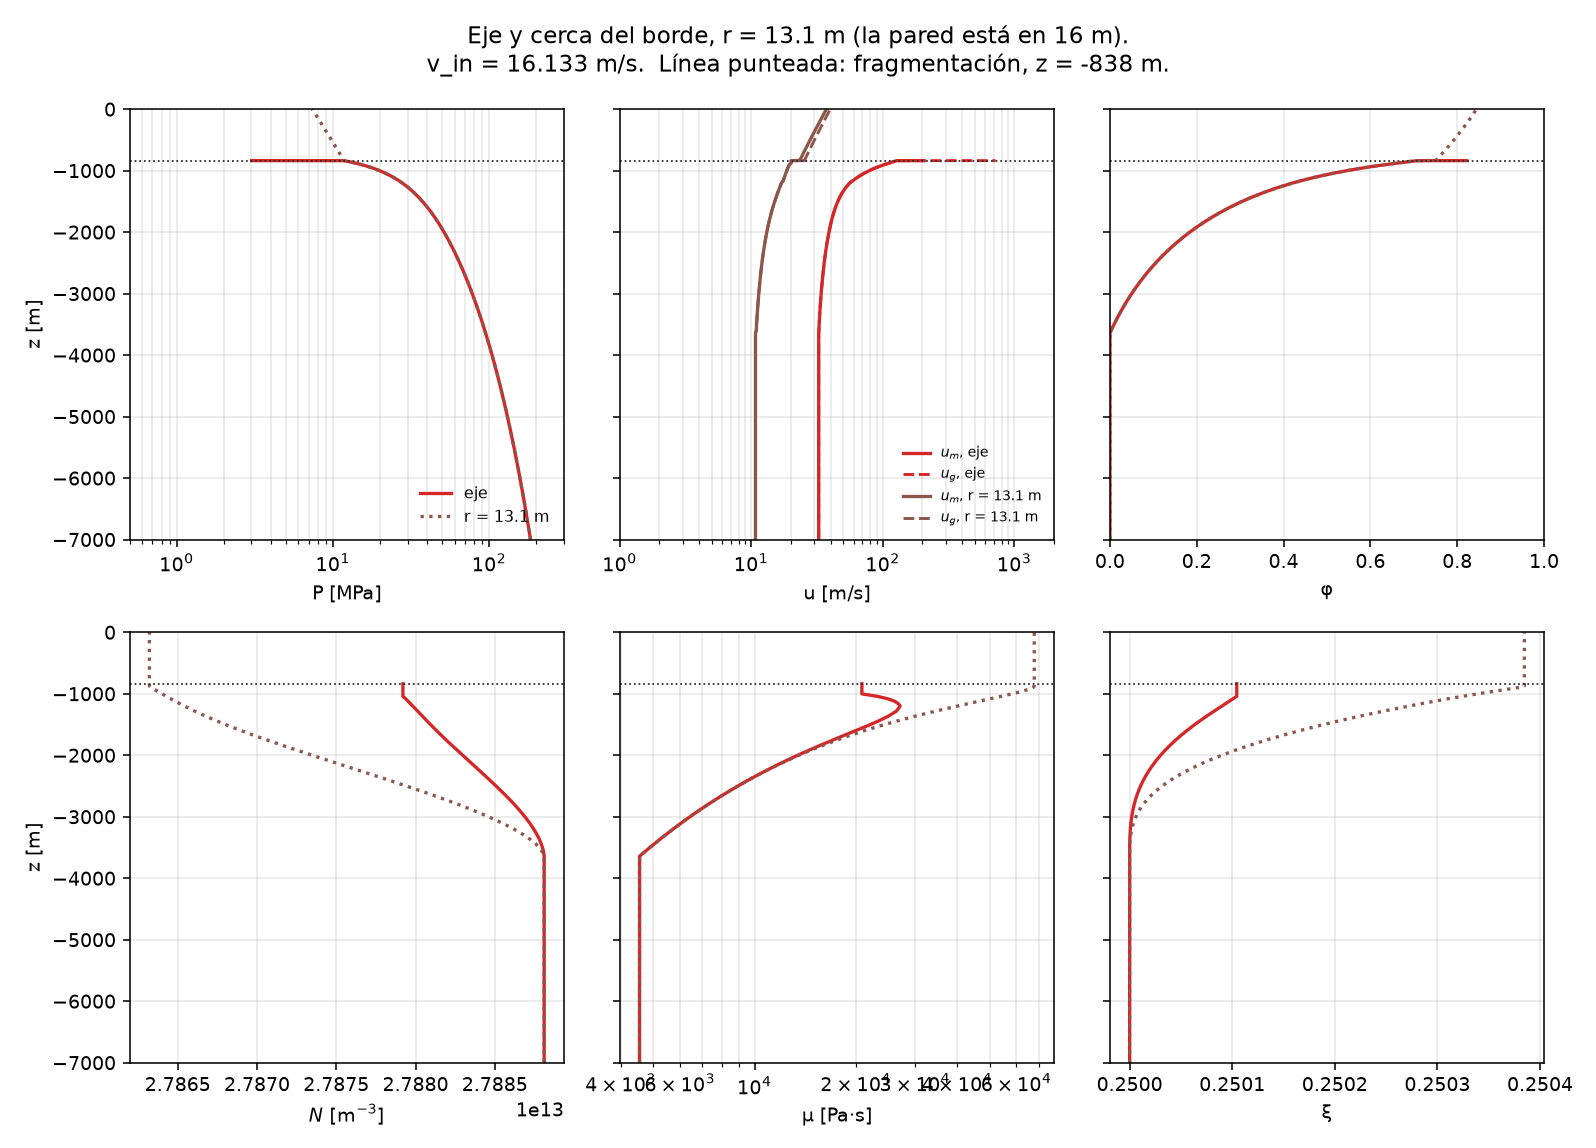
\includegraphics[width=\textwidth]{perfiles-eje-borde.png}
\caption{Columna con $\vin=16{,}133\ms$. El eje se corta en
$z=-837\,\mathrm{m}$ al llegar $u_g$ a $757\ms$. El radio
$r=13{,}1\,\mathrm{m}$ alcanza la boca a $80\ms$ y $6{,}95\MPa$.}
\label{fig:eje-borde}
\end{figure}

\subsection{Diferencias hacia atrás}

\paragraph{Variables del nivel nuevo.}
$u_{m,j}$, $u_{g,j}$, $P_j$, $\varphi_j$. El nivel $j-1$ es dato.
Entra $L_{r,j}$.

En cada paso de altura $h$ se resuelve el sistema
\begin{align}
\label{eq:fd-frag}
\rho_m\frac{u_{m,j}^{2}-u_{m,j-1}^{2}}{2h}
+\frac{P_j-P_{j-1}}{h}+\rho_m g
-\frac{F_{mg,j}}{1-\varphi_j}
&=0,
\\
\rho_g\frac{u_{g,j}^{2}-u_{g,j-1}^{2}}{2h}
+\frac{P_j-P_{j-1}}{h}+\rho_g g
+\frac{F_{mg,j}}{\varphi_j}
-\frac{L_{r,j}}{\varphi_j}
&=0.
\end{align}
Cerca de $u_g=c_s$ el paso baja hasta $10^{-5}\,\mathrm{m}$. Con el
$\vin$ del tiro, el eje se detiene en $z=-837{,}3\,\mathrm{m}$, con
$P=7{,}23\MPa$, $u_g=718\ms$, $u_m=47\ms$ y $\varphi=0{,}864$.
La marcha de Euler de la figura~\ref{fig:eje-borde} corta el mismo
eje en $z=-837\,\mathrm{m}$, con $u_g=757\ms$ y $P=7{,}15\MPa$.

\begin{figure}[ht]
\centering
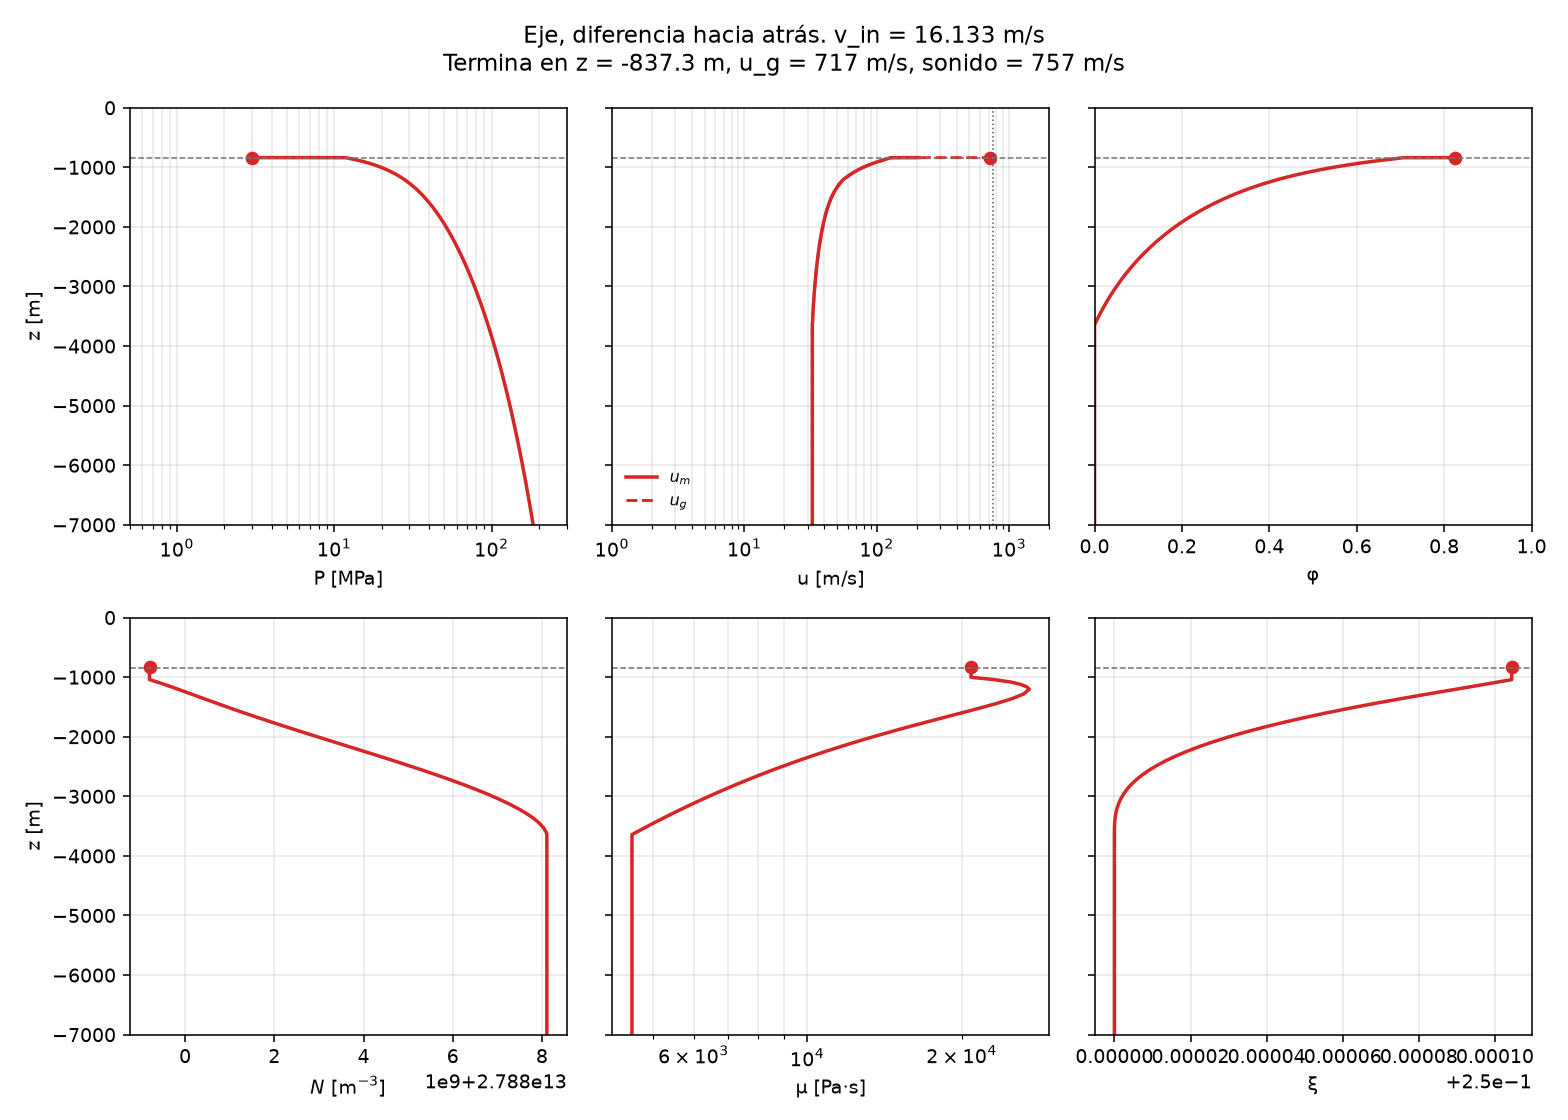
\includegraphics[width=\textwidth]{perfiles-eje-fd.png}
\caption{Eje con \eqref{eq:fd-frag}. $z_f=-838\,\mathrm{m}$,
$P_f=10\MPa$, $u_{g,f}=51\ms$. Último nivel en
$z=-837{,}3\,\mathrm{m}$, con $u_g=718\ms$ y $P=7{,}23\MPa$.}
\label{fig:fd}
\end{figure}

\subsection{Radios que siguen}

Cuando un nodo llega a $u_g$ sónica sale del sistema
\eqref{eq:fd-frag} y el resto sigue. Los cinco radios interiores
se congelan entre $z=-837{,}3\,\mathrm{m}$ y $z=-153\,\mathrm{m}$.
Los dos exteriores llegan a la boca, con presiones de $6{,}9$ y
$7{,}4\MPa$. Cada radio termina con su propia $P$.

\begin{table}[ht]
\centering
\caption{Último nivel de cada radio en \eqref{eq:fd-frag}, con
$\vin=16{,}133\ms$.}
\label{tab:radios}
\begin{tabular}{@{}rrrrp{4.8cm}@{}}
\toprule
$r$ [m] & $z$ [m] & $P$ [\MPa] & $u_g$ [\ms] & estado \\
\midrule
$0{,}0$  & $-837{,}3$ & $7{,}23$ & $718$ & sónico \\
$2{,}9$  & $-837{,}2$ & $7{,}28$ & $699$ & sónico \\
$5{,}8$  & $-836{,}0$ & $8{,}05$ & $557$ & sónico \\
$8{,}7$  & $-671{,}6$ & $9{,}48$ & $160$ & sónico \\
$10{,}2$ & $-153{,}1$ & $8{,}86$ & $92$  & sónico \\
$11{,}6$ & $0{,}0$    & $6{,}86$ & $74$  & en la boca \\
$13{,}1$ & $0{,}0$    & $7{,}39$ & $40$  & en la boca \\
\bottomrule
\end{tabular}
\end{table}

\begin{figure}[ht]
\centering
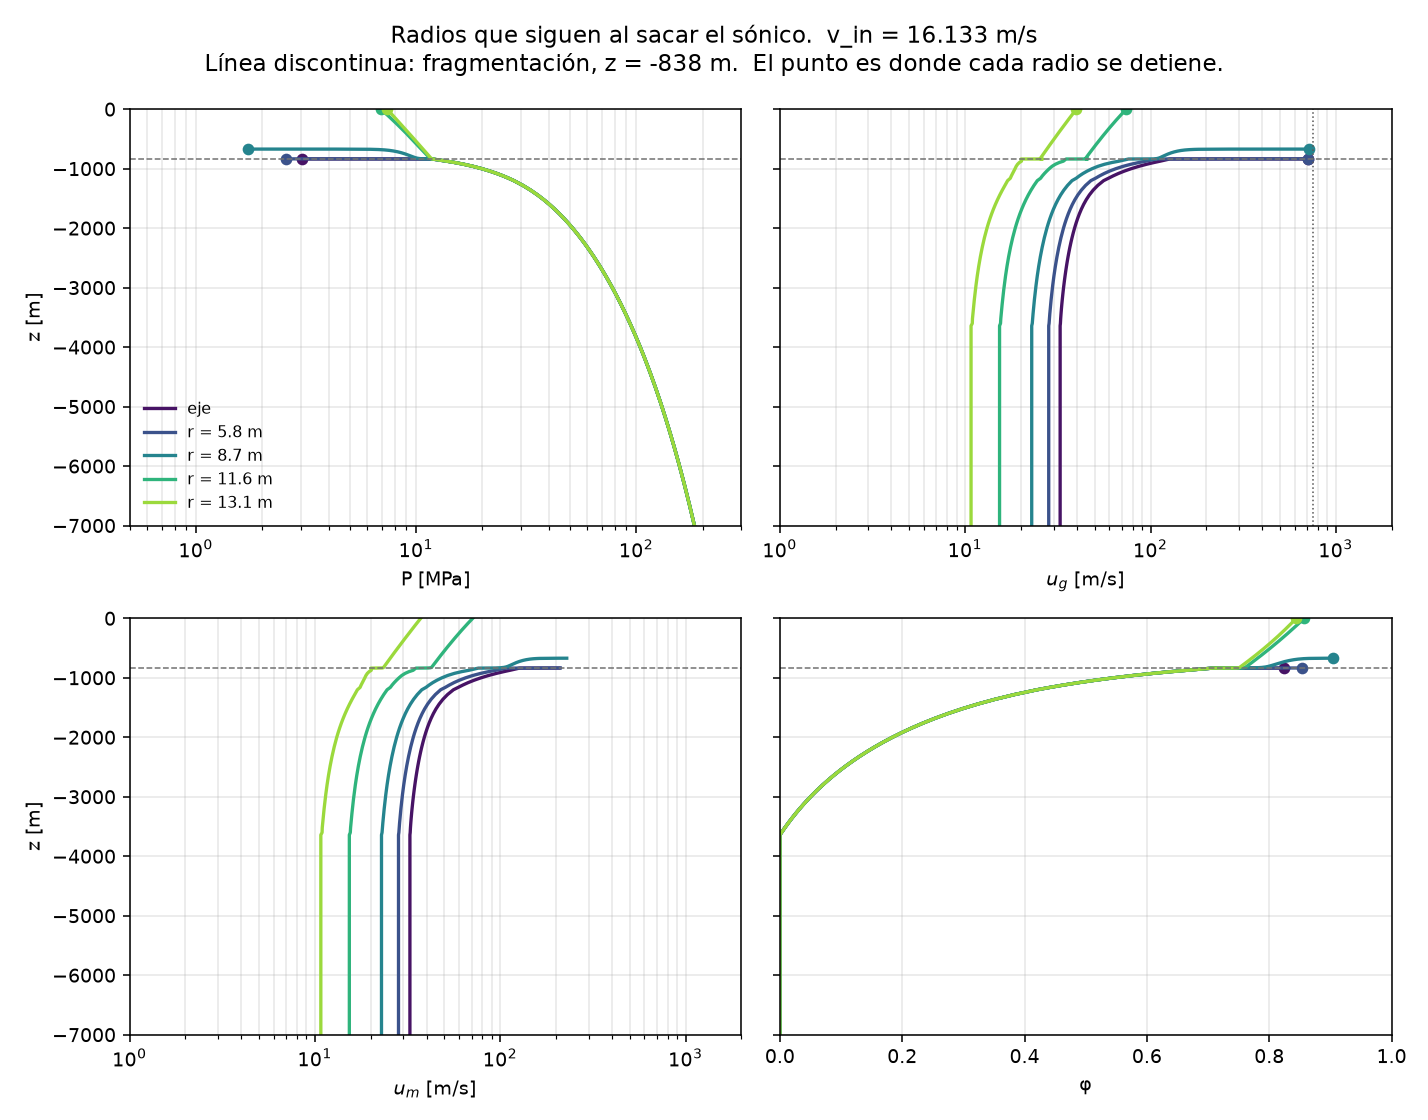
\includegraphics[width=\textwidth]{radios-siguen-fd.png}
\caption{Siete radios con \eqref{eq:fd-frag}. Las curvas interiores
se cortan al acercarse a $c_s$. Los radios $r=11{,}6\,\mathrm{m}$ y
$r=13{,}1\,\mathrm{m}$ siguen hasta $z=0$.}
\label{fig:radios}
\end{figure}

Con $P=P(r,z)$, la componente radial \eqref{eq:P-2d} deja de dar
$\p P/\p r=0$. Entran $u_{m,r}$ y $u_{g,r}$, y la masa vuelve a ser
\eqref{eq:masa-2d}: el caudal $q(r)$ de \eqref{eq:q-f} deja de ser
constante en $z$ en cuanto hay flujo de una corona a otra. Las
marchas de esta sección usan $u_{m,r}=u_{g,r}=0$.

\section{Unidimensional en el tiempo}
\label{sec:tiempo}

El dominio sigue siendo $z\in[H,0]$, ahora con $t\ge 0$. La sección
es constante y el flujo es isotermo, como en la
sección~\ref{sec:1d}. El estado es
$(P,\varphi,N,\xi,u_m,u_g)(z,t)$. La densidad del gas sigue siendo
\eqref{eq:eos}. La suma de las dos masas ya no deja un caudal
constante: $q=q(z,t)$.

\subsection{Masa}

\paragraph{Variables.}
$\varphi$, $u_m$, $u_g$ y el caudal
$q(z,t)=\rho_m(1-\varphi)\,u_m+\rho_g\,\varphi\,u_g$.
Entran $\rho_g(P)$ y la tasa de exsolución $\Gamma$.

\begin{align}
\label{eq:masa-t}
\frac{\p}{\p t}\bigl[\rho_m(1-\varphi)\bigr]
+\frac{\p}{\p z}\bigl[\rho_m(1-\varphi)\,u_m\bigr]
&=-\Gamma,
\\
\frac{\p}{\p t}\bigl[\rho_g\,\varphi\bigr]
+\frac{\p}{\p z}\bigl[\rho_g\,\varphi\,u_g\bigr]
&=\Gamma.
\end{align}
$\rho_m$ se toma constante, como en el conducto unidimensional
estacionario. Al sumar \eqref{eq:masa-t} la exsolución se cancela
y queda la masa total,
\begin{equation}
\label{eq:q-t}
\frac{\p\rho_{\mathrm{mix}}}{\p t}+\frac{\p q}{\p z}=0,
\qquad
\rho_{\mathrm{mix}}=\rho_m(1-\varphi)+\rho_g\,\varphi.
\end{equation}
Con $\p/\p t=0$, \eqref{eq:q-t} devuelve $q=\mathrm{const}$, que es
\eqref{eq:q}.

\subsection{Momento}

\paragraph{Variables.}
$P$, $u_m$, $u_g$. Entran $\varphi$, $F_{mg}$, $F_{mw}$ y $F_{gw}$,
con la misma viscosidad \eqref{eq:mu} y el mismo arrastre por
régimen de la sección~\ref{sec:1d}.

\begin{align}
\label{eq:mom-t}
\rho_m(1-\varphi)\Biggl(
\frac{\p u_m}{\p t}+u_m\frac{\p u_m}{\p z}
\Biggr)
&=
-(1-\varphi)\frac{\p P}{\p z}
-\rho_m(1-\varphi)\,g
+F_{mg}-F_{mw},
\\
\rho_g\,\varphi\Biggl(
\frac{\p u_g}{\p t}+u_g\frac{\p u_g}{\p z}
\Biggr)
&=
-\varphi\frac{\p P}{\p z}
-\rho_g\,\varphi\,g
-F_{mg}-F_{gw}.
\end{align}
Con $\p/\p t=0$, \eqref{eq:mom-t} es \eqref{eq:mom-1d}. $F_{mw}$ se
apaga en el tramo fragmentado y ahí aparece $F_{gw}$, igual que en
el estacionario.

\subsection{Número de burbujas y cristales}

\paragraph{Variables.}
$N$ y $\xi$. Entran $u_m$, $\Gamma_N$ y $\Gamma_\xi$, las mismas
tasas \eqref{eq:GammaN} y \eqref{eq:Gammaxi}.

\begin{align}
\label{eq:Nxi-t}
\frac{\p N}{\p t}+u_m\frac{\p N}{\p z}
&=\Gamma_N(P,\varphi,N,\xi),
\\
\frac{\p \xi}{\p t}+u_m\frac{\p \xi}{\p z}
&=\Gamma_\xi(P,\xi).
\end{align}
Después de fragmentar las dos tasas se anulan, así que $N$ y $\xi$
solo se advectan. En el estacionario, \eqref{eq:Nxi-t} dividido por
$u_m$ es \eqref{eq:N-1d}--\eqref{eq:xi-1d}.

\subsection{Exsolución}

\paragraph{Variables.}
$\Gamma$, o bien $\varphi$ cuando se reemplaza la masa por una
relajación. Entran $P$, $\xi$ y $\tau_{\mathrm{relax}}$.

En equilibrio, $n=n(P,\xi)$ es Henry \eqref{eq:henry} en cada
$(z,t)$, y $\Gamma$ es la tasa que mantiene el agua disuelta sobre
esa curva. El límite estacionario con $u_m=u_g$ devuelve el volumen
\eqref{eq:phi-noslip}.

El integrador que ya corre no evoluciona las dos masas. Evoluciona
$\varphi$ hacia el volumen de equilibrio, con $u_m$ la velocidad de
la mezcla en ese instante:
\begin{equation}
\label{eq:relax}
\frac{\p\varphi}{\p t}+u_m\frac{\p\varphi}{\p z}
=\frac{\varphi_{\mathrm{eq}}(P,\xi)-\varphi}{\tau_{\mathrm{relax}}}.
\end{equation}
$\varphi_{\mathrm{eq}}$ es \eqref{eq:phi-noslip}. El valor usado es
$\tau_{\mathrm{relax}}=200\,\mathrm{s}$. Si
$\tau_{\mathrm{relax}}\to 0$, $\varphi$ queda en
$\varphi_{\mathrm{eq}}$ en cada paso.

\subsection{Condiciones}

Hace falta un dato en toda la columna y un par base--boca.

\paragraph{Inicial, $t=0$.}
$(P,\varphi,N,\xi,u_m,u_g)(z,0)$ en $[H,0]$. Dos datos ya usados:
la columna estacionaria del mismo caso, explosiva o efusiva; y la
columna sin burbujas, $\varphi=0$, $\xi=\xi_0$, $N=N_0$, con el
caudal que lleva $P(0)$ a $P_{\mathrm{atm}}$. Sobre la segunda, las
burbujas crecen en la escala $\tau_{\mathrm{relax}}$.

\paragraph{Base, $z=H$, para todo $t$.}
\begin{equation}
\label{eq:base-t}
P(H,t)=P_{\mathrm{lit}}+\Delta P(t),
\qquad
\xi(H,t)=\xi_0,
\qquad
N(H,t)=N_0.
\end{equation}
$\varphi(H,t)$ es el volumen de Henry si la cámara está saturada, y
$0$ si el agua sigue disuelta. $\Delta P$ constante es el borde del
estacionario. Si $\Delta P$ lo entrega una cámara de volumen
$V_{\mathrm{cam}}$,
\begin{equation}
\label{eq:camara}
C_{\mathrm{cam}}\frac{\dd P_{\mathrm{cam}}}{\dd t}
=Q_{\mathrm{entrada}}-\mathrm{MER}(P_{\mathrm{cam}}),
\qquad
C_{\mathrm{cam}}
=\rho_m V_{\mathrm{cam}}\Biggl(\frac{1}{K_m}+\frac{1}{K_{\mathrm{cam}}}\Biggr).
\end{equation}
$P(H,t)=P_{\mathrm{lit}}+P_{\mathrm{cam}}(t)$. En el recorte de
lubricación, con $V_{\mathrm{cam}}=50\,\mathrm{km}^3$, el tiempo
$C_{\mathrm{cam}}/G$ de esa cámara es $5{,}83\,\mathrm{h}$.

\paragraph{Boca, $z=0$.}
Se impone una sola condición, la del estacionario:
\begin{equation}
\label{eq:boca-t}
P(0,t)=P_{\mathrm{atm}}
\quad\text{o}\quad
u_g(0,t)=c_s=\sqrt{\Rv T}.
\end{equation}
Mientras $u_g<c_s$, el dato es la presión atmosférica y el caudal
$q(t)$ es el que la cumple. Cuando el gas llega a $c_s$, el dato
pasa a ser la velocidad sónica y $P(0,t)$ sale de la integración.
$u_m$, $N$ y $\xi$ no se imponen en la boca: el flujo sale del
dominio. En la base tampoco se impone la velocidad de salida; el
caudal de entrada queda atado a \eqref{eq:boca-t}.

El integrador en \texttt{RIconduit1D\_transient.py} usa la primera
opción de \eqref{eq:boca-t} en todo el cálculo: en cada $t$ recalcula
un $q(t)$, uniforme en $z$, tal que $P(0,t)=P_{\mathrm{atm}}$. Con
ese $q$ y con los perfiles $\varphi$, $N$ y $\xi$ del instante,
$P$, $u_m$ y $u_g$ salen del balance de momento sin el término
$\p/\p t$. Avanza en el tiempo \eqref{eq:relax} y \eqref{eq:Nxi-t},
con diferencias hacia atrás en $z$ y RK4, paso
$\Delta t\le 0{,}4\,\Delta z/\max(u_m,u_g)$. El umbral de
fragmentación va fijo en $0{,}75$ salvo que se le pase el
$\varphi_{\mathrm{crit}}$ del estacionario. Los nodos de la base
quedan en el valor inicial de $\varphi$, $N$ y $\xi$.

\subsection{Cuándo pesa el término en el tiempo}

La comparación de escalas es el número de Deborah
$\mathrm{De}=\tau_{\mathrm{conducto}}/\tau_{\mathrm{forzamiento}}$.
En el recorte de lubricación de Calbuco se midió
$\tau_{\mathrm{hidr}}=8\,\mathrm{s}$ para la respuesta del caudal
tras un escalón de presión, $\tau_{\mathrm{resid}}=6\,\mathrm{min}$
de residencia y $\tau_{\mathrm{cam}}=5{,}83\,\mathrm{h}$. El drenaje
de esa cámara tiene $\mathrm{De}=5{,}7\times 10^{-4}$, y el caudal
obtenido con la columna estacionaria del $\Delta P(t)$ instantáneo
difiere $0{,}08\pc$ del integrado en el tiempo. El error llega a
$1\pc$ cuando $\mathrm{De}\approx 0{,}09$, esto es, forzamientos de
menos de unos $90\,\mathrm{s}$.

Con esas escalas, el término $\p/\p t$ del conducto entra en cuatro
situaciones.

\begin{enumerate}[leftmargin=1.2em,itemsep=0.35em]
\item Apertura. La columna parte en $\varphi=0$ y el gas exsuelve en
$\tau_{\mathrm{relax}}$. El nivel $z_f(t)$ se mueve. Una columna
estacionaria no trae ese frente.
\item Un cambio de $\Delta P$ en menos de un minuto. Ahí
$\mathrm{De}\gtrsim 0{,}1$ y el caudal se aparta del estacionario
del $\Delta P$ de ese instante.
\item Cristalización durante un drenaje de horas. $\tau_c=2\,\mathrm{h}$
está en el rango $10^{4}$--$10^{6}\,\mathrm{s}$ de los microlitos.
Con $\tau\sim 10^{4}\,\mathrm{s}$ y una fase de $6\,\mathrm{h}$,
$\mathrm{De}\approx 0{,}5$: $\xi(z,t)$ no es el perfil estacionario
del $\Delta P(t)$ instantáneo. La exsolución en desequilibrio, con
$\tau_{\mathrm{relax}}$ entre $10^{1}$ y $10^{3}\,\mathrm{s}$, cae
en la misma situación si el forzamiento es de ese orden.
\item Un domo cíclico. El período lo fija la cinética de
cristalización o de escape de gas ($10^{3}$--$10^{5}\,\mathrm{s}$),
así que la evolución es la de \eqref{eq:Nxi-t} y \eqref{eq:relax}.
\end{enumerate}

En el drenaje de Calbuco mirado solo por la hidráulica, con
$\tau_{\mathrm{cam}}$ de horas, la sucesión de columnas
estacionarias de $\Delta P(t)$ ya da el $\mathrm{MER}(t)$.

\section{Operador directo}

Las marchas de arriba, con un $\vin$ aceptado por \eqref{eq:boca},
leen el caudal $Q$ en la boca. El dato de borde que se deja libre
es un escalar de la base,
\begin{equation}
\label{eq:F}
\mathcal{F}(\theta)=Q,
\qquad
\theta=\Delta P
\quad\text{o}\quad
\theta=c_0,
\end{equation}
uno por vez. $\Delta P$ entra en $P(H)$. $c_0$ entra en Henry,
\eqref{eq:henry} y \eqref{eq:nad}. En el tiempo de la
sección~\ref{sec:tiempo} el dato de la boca es la función
$Q(t)$, con $\Delta P(t)$ dado por \eqref{eq:base-t} o por la
cámara \eqref{eq:camara}.

\end{document}
